\section[The coherent photon source and beamline]{The coherent photon source and beamline \label{sec:beamline}}
%{\color{red}General comment: As we haggle in the beamline group over the level of detail required for this section, it is worth bearing in mind that a longer-form paper dedicated to the beamline is also on our to-do list.  Material and detail felt to be excessive for this document can spill over into that paper}

\begin{table}[tbp]
\begin{center}
\caption
[Design properties of the electron beam]
{Electron beam parameters. 
The emittance, energy spread and
related parameters are estimates
based on a model of the transport line from
the accelerator to the Hall D radiator.
The dimensions of the beam spot at the position of 
the radiator are directly measured, and vary about the
stated values by $\pm 30\%$
depending on beam conditions. 
Values for image size at collimator,
obtained by projection of the electron beam
spot convergence forward to the position of
the primary photon collimator, have relative
uncertainties of 50\%.}
\label{tab:elecprop}
\begin{tabular}{|l|c|}
\hline\hline
parameter & design results \\
\hline
energy & 12~GeV \\
%electron polarization & available \\
energy spread, RMS & $2.2$~MeV \\
transverse $x$ emittance & 2.7~mm$\cdot\mu$rad \\
transverse $y$ emittance & 1.0~mm$\cdot\mu$rad \\
$x$ spot size at radiator, RMS & 1.1~mm \ \\
$y$ spot size at radiator, RMS & 0.7~mm \ \\
$x$ image size at collimator, RMS & 0.5~mm \\
$y$ image size at collimator, RMS & 0.5~mm \\
image offset from collimator axis, RMS & 0.2~mm \\
distance radiator to collimator & 75.3~m \\
\hline\hline
\end{tabular}
\end{center}
\end{table}

\subsection{CEBAF electron beam \label{sec:ebeam}}
The Continuous Electron Beam Accelerator Facility (CEBAF) has a race track configuration with two parallel linear accelerators based on superconducting radio frequency (RF) technology \cite{Leemann:2001dg}. The machine operates at 1.497 GHz and delivers beam to Hall D at 0.249.5~GHz.\footnote{Hall D beam at 499 MHz is possible, but not usual.} Precise timing signals for the accelerator beam bunches are available to the experiment and are used to determine the time of individual bunches passing through the target. The nominal properties for the CEBAF electron beam to the Tagger Hall are listed in Table\,\ref{tab:elecprop}.

\subsection{Hall D photon beam \label{sec:gbeam}}
The Hall D complex, described in Section \ref{sec:gluexexperiment:complex} and shown schematically in Fig.~\ref{fig:beam:Draw_beamline}, includes a dedicated Tagger Hall, an associated collimator cave, and Experimental Hall D itself. A linearly-polarized photon beam is created using the process of coherent bremsstrahlung \cite{timm1969,LIVINGSTON2009205} when the electron beam passes through an oriented diamond radiator at the upstream end of the Tagger Hall.
The electron beam position at the radiator is monitored and controlled using beam position monitors, named 5C11 and 5C11B, which are located at the end of the accelerator tunnel just upstream of the Tagger Hall. (The position of 5C11B is indicated in Figure \ref{fig:beam:Draw_beamline}.)
%The position of the beam on the collimator is initially set by adjusting small corrector magnets at this location.
The CEBAF electron beam is tuned 
so as to be converging as it passes through the radiator, ideally
so that the electron beam forms a virtual focus at the collimator 
located 75\,m downstream of the radiator.
At the collimator, the virtual spot size ($\sim$ 0.5\,mm) is small compared to the cm-scale size of the photon beam on the face of the collimator,
such that a cut on photon position at the collimator is effectively a cut on photon emission angle at the radiator. 
The convergence
properties of the electron beam are measured independently 
in X (vertical) and Y (horizontal) 
by scanning vertical (horizontal) wires 
through the beam and measuring the induced current on the wire (or the scattered beam intensity) as a function of position; the wire scanners are referred to as ``harps".
Examples of the horizontal and vertical convergence of the electron beam envelope (undeflected by the tagger magnet)
measured using harp scans and projected downstream along the beamline are shown in Fig.\,\ref{fig:beam:convergence}.

\begin{figure}[tbp]
\begin{center}
 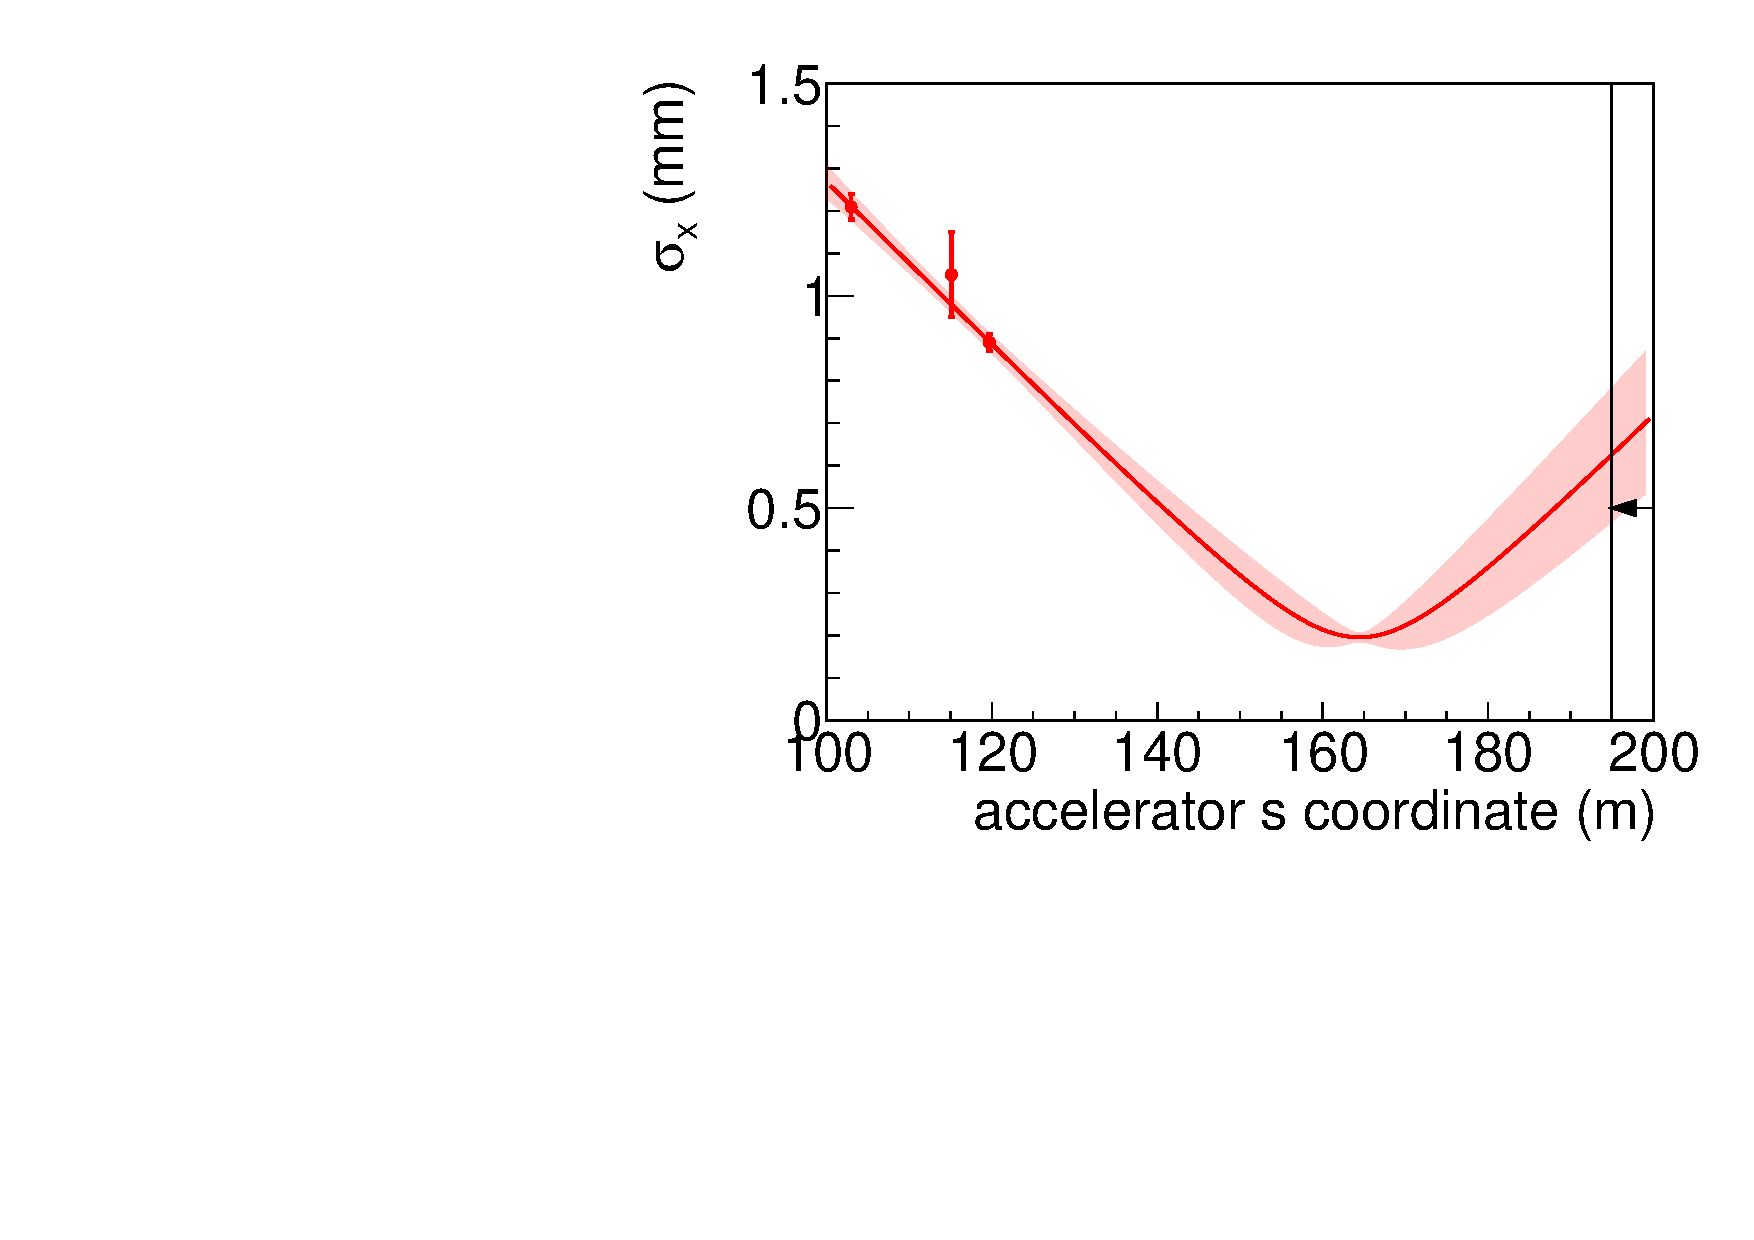
\includegraphics[clip=true,width=0.49\linewidth]{figures/harp-x-767755.pdf}
 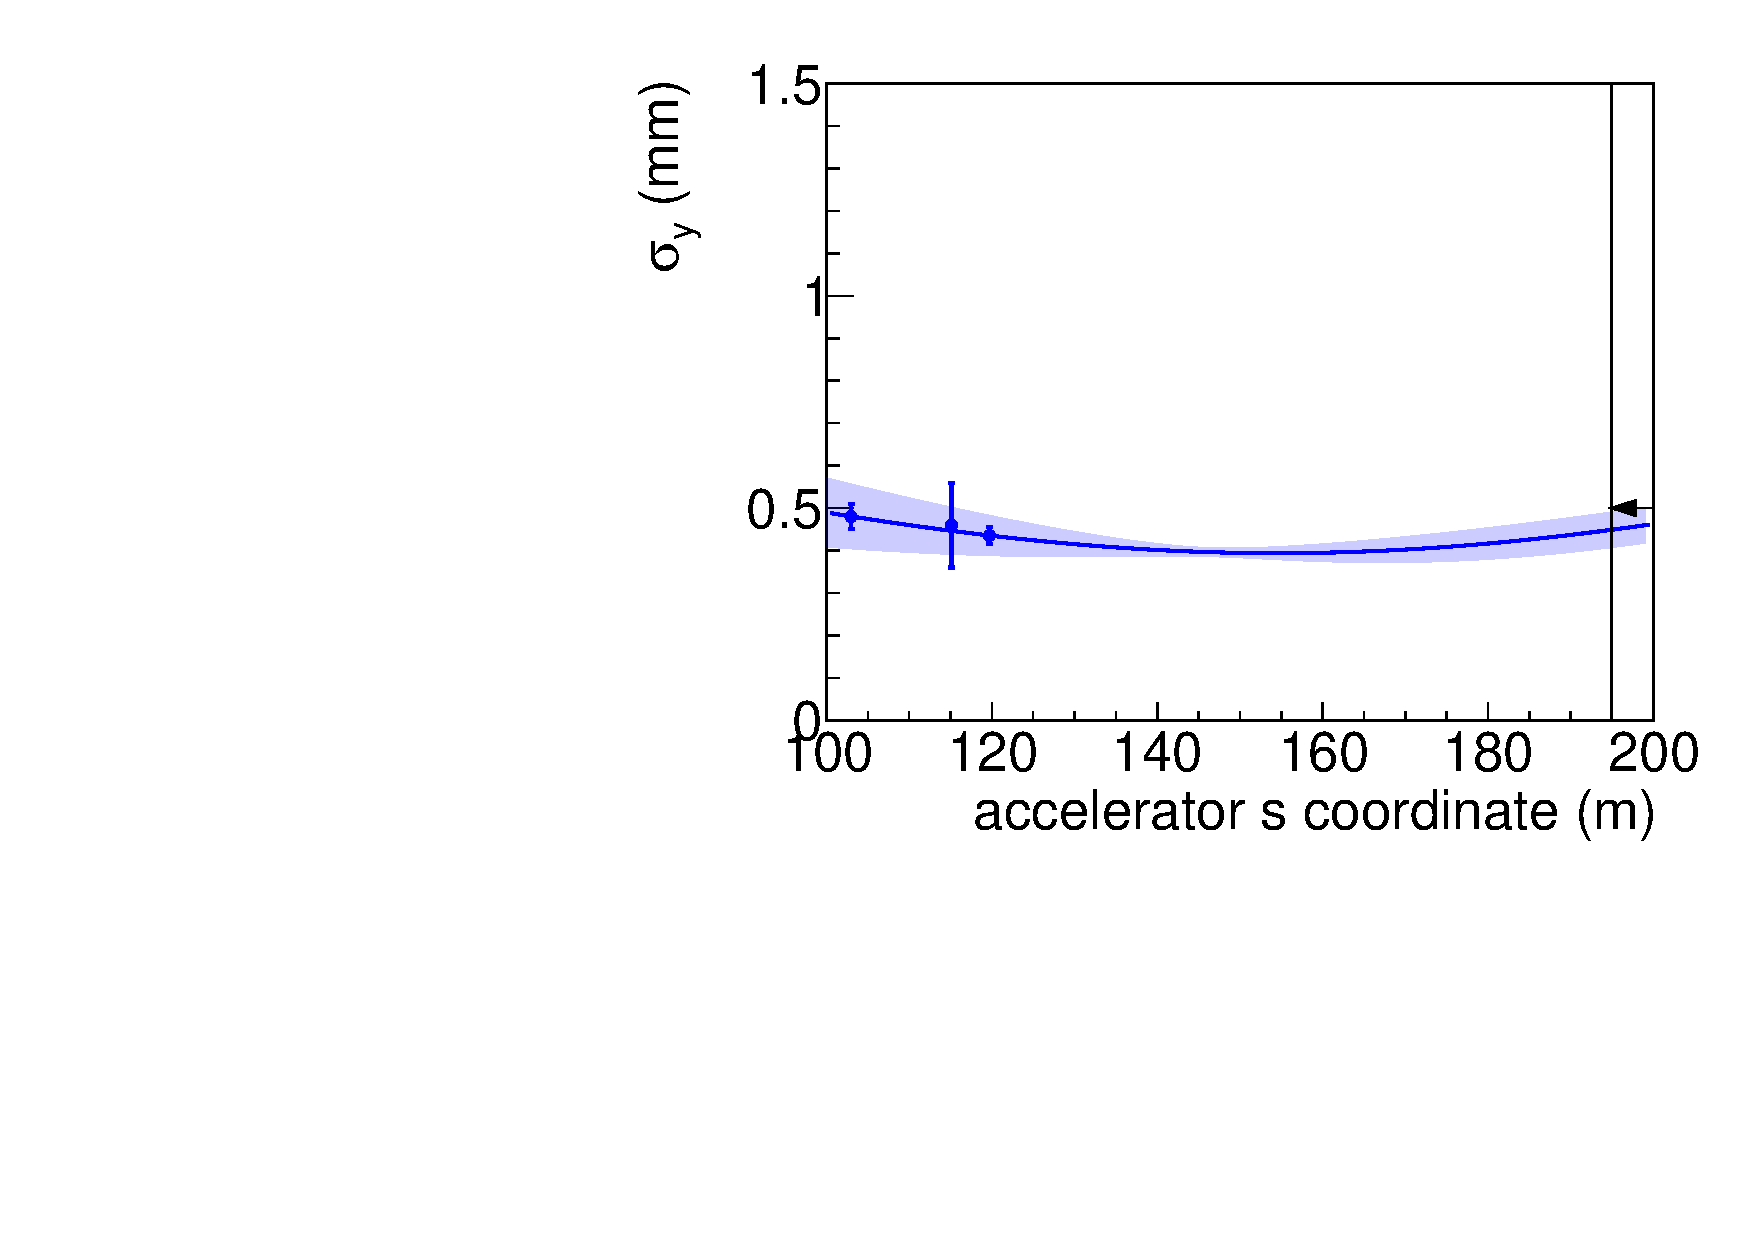
\includegraphics[clip=true,width=0.49\linewidth]{figures/harp-y-767755.pdf}
\end{center}
\caption{(Color online) Measurements of the root-mean-square width of the electron beam 
in horizontal (left)
and vertical (right) projections as a function of position along the beamline, based on
harps scans (data points) of the electron beam. The radiator position is just upstream
of the third data point. The primary collimator position is marked by the vertical line
indicated by the arrow. The curve downstream of the radiator is an extrapolation from
the measured data points, with extrapolation uncertainty indicated by the shaded regions.
        }
\label{fig:beam:convergence} 
\end{figure}

The photon beam position on the collimator is monitored using an
the active collimator positioned just upstream of the primary photon beam collimator
(described below in section \ref{sec:coll}). 
The stability of the beam is maintained during normal
operation of the beamline by a feedback system that locks the position of the electron
beam at the 5C11B beam profile monitor and, consequently, the photon beam at the active collimator. The stability of the electron
beam current and position is monitored using an independent beam position monitor
(named AD00C and shown in Fig.\,\ref{fig:beam:Draw_beamline}) 
located immediately upstream of the electron dump.

%\begin{figure}[t]
%\begin{center}
%   %\includegraphics[viewport=1 1 790 %540,clip,angle=0,width=0.98\linewidth]{figs/mainmachine_beamline_dwg}
%\end{center}
%\caption{Schematics of the accelerator and the beam extraction system.
%        }
%\label{fig:beam:cebaf-dwg} 
%\end{figure}

\begin{figure}[t]
\begin{center}
%   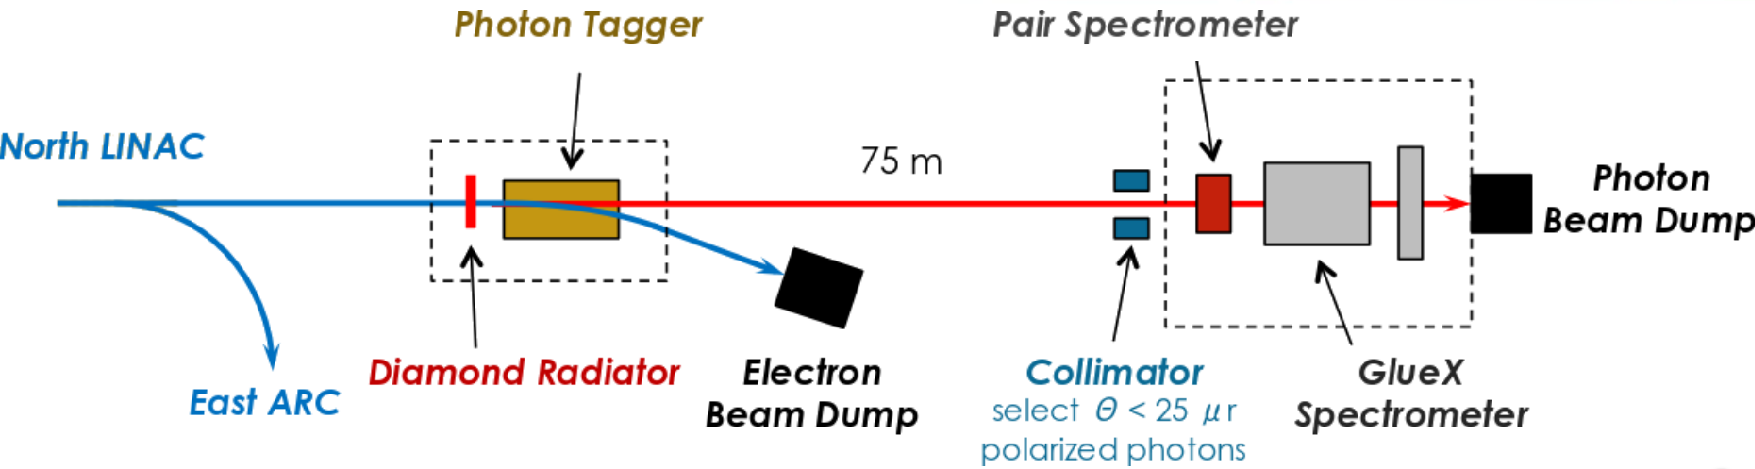
\includegraphics[clip=true,width=0.98\linewidth]{figures/gx_beamline_0}https://www.overleaf.com/6913428728kzgcdrhmtbjj
 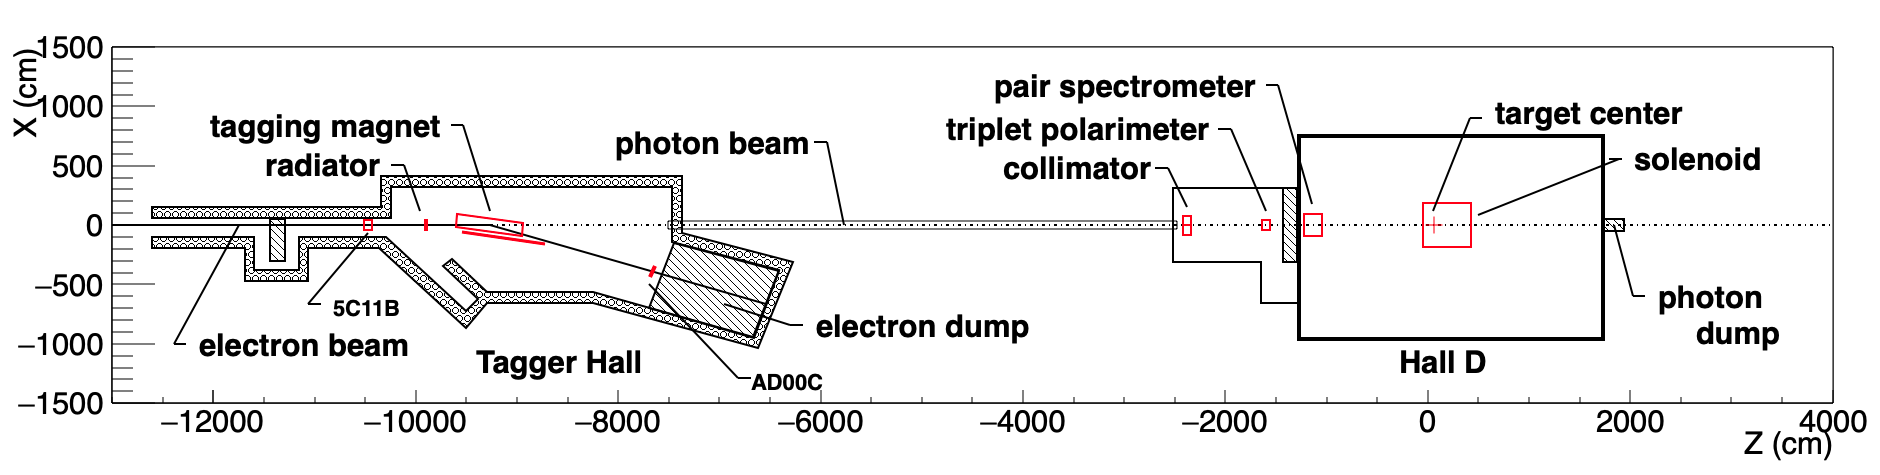
\includegraphics[clip=true,width=0.98\linewidth]{figures/Draw_beamline.png}
\end{center}
\caption{Schematic layout of the Hall D complex, showing the Tagger Hall, Hall D, and
several of the key beamline devices.
Also indicated are the locations of the 5C11B and AD00C beam position monitors.
        }
\label{fig:beam:Draw_beamline} 
\end{figure}

The linearly-polarized photon beam is produced in a radiator placed in the electron beam just upstream of the
tagger (section \ref{sec:tag}). A properly aligned 20--60\,$\mu m$ thick diamond crystal
radiator produces
linearly-polarized photons via coherent brems\-strah\-lung in enhancements that \cite{timm1969,LIVINGSTON2009205},
appear as peaks at certain energies in the brems\-strah\-lung intensity spectrum (Fig.\,\ref{fig:beam:gx3102_pi0etaAsym2016_fig0_beam}), superimposed upon the ordinary brems\-strah\-lung
continuum spectrum.
The energies of the coherent photon peaks and the degree of polarization in each of those peaks depend on the crystal orientation with respect to the incident electron beam.
Adjustment of the orientation of the diamond crystal with respect to the incoming
electron beam permits production of essentially any coherent photon peak energy up to that of the energy of the incident electron beam, as well as the
degree or direction of linear polarization.
A choice of 9 GeV for the primary peak energy, corresponding to 40\% peak linear polarization,
was found to be optimum for the \GX{} experiment with a 12 GeV incident electron beam.

\begin{figure}[tbp]
\begin{center}
 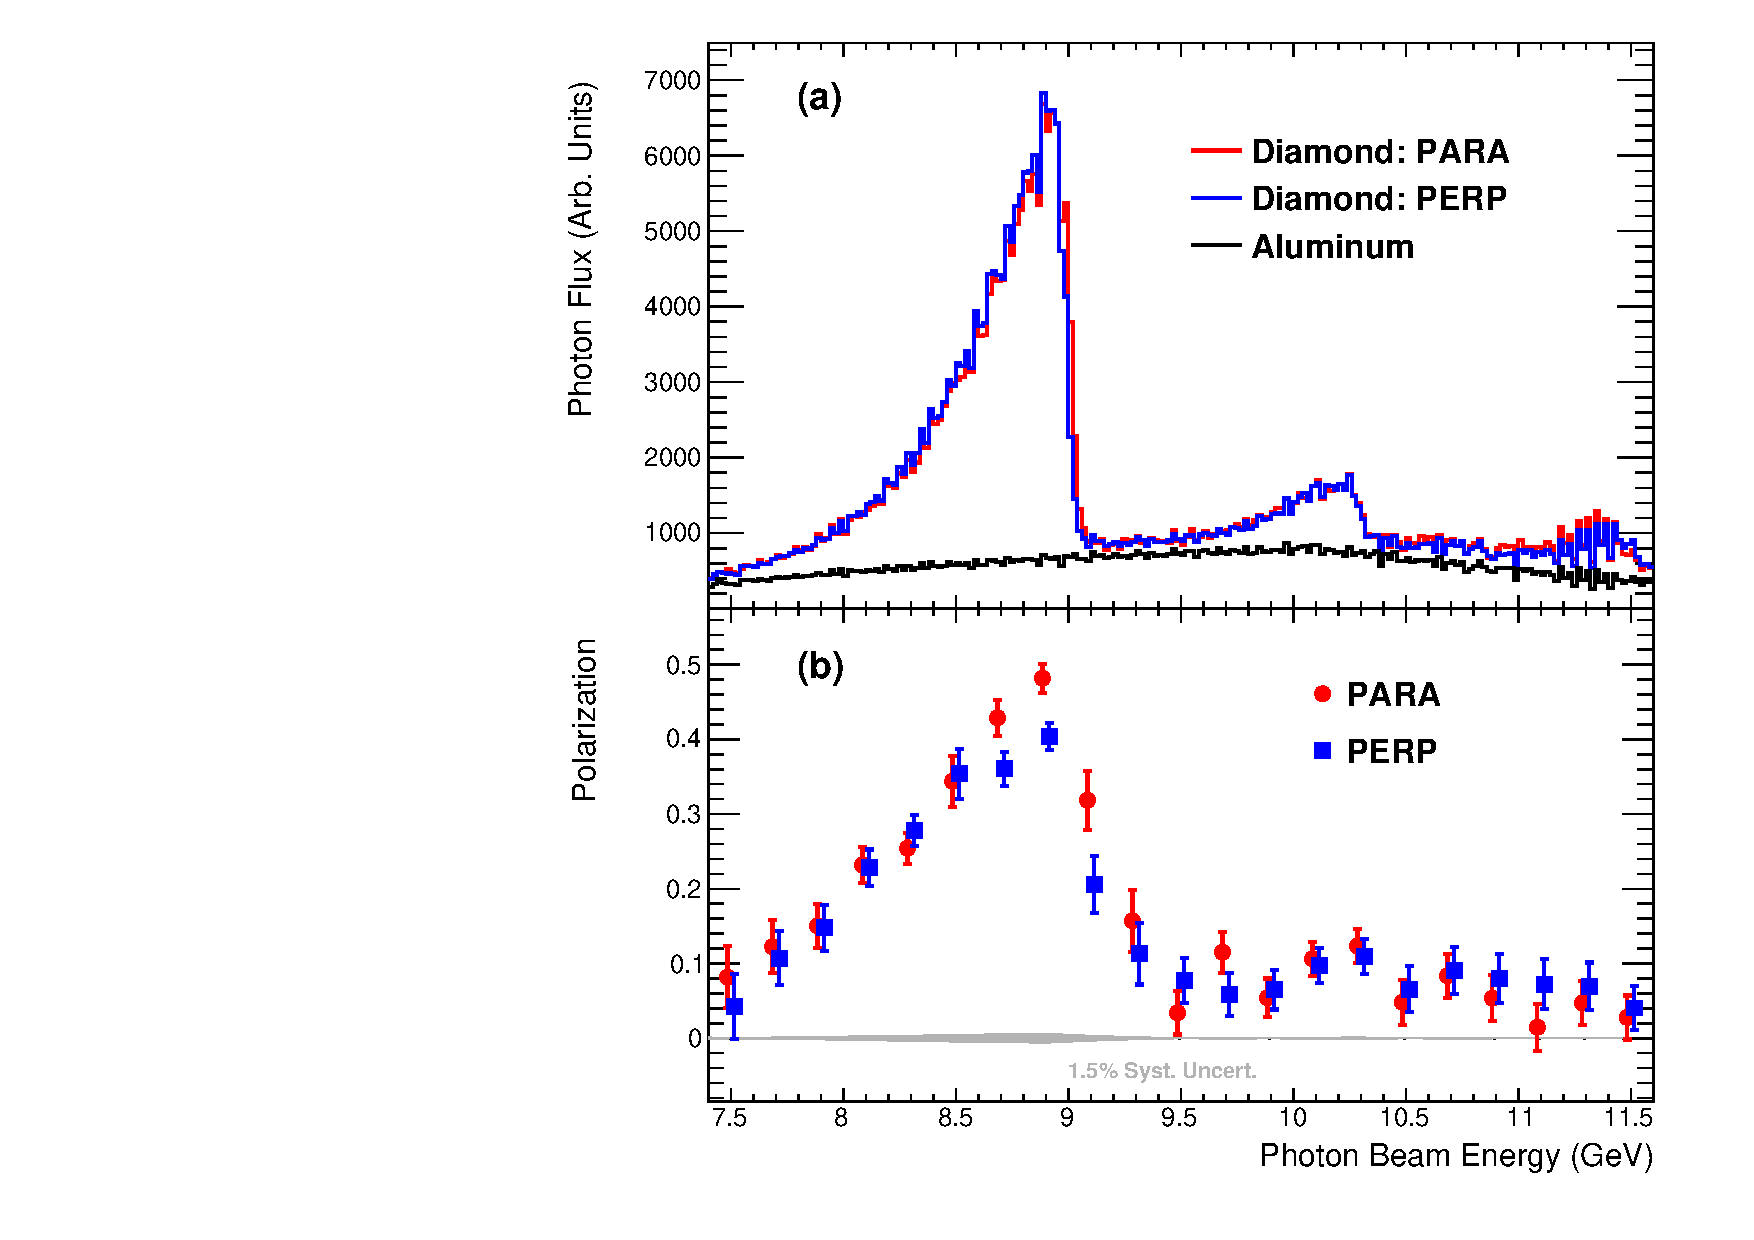
\includegraphics[clip=true,width=0.5\linewidth]{figures/gx3102_pi0etaAsym2016_fig0_beam.pdf}
\end{center}
\caption{(color online) (a) Photon beam intensity versus energy as measured by the pair spectrometer
(not corrected for instrumental acceptance).  (b) Photon beam polarization as a function of beam energy,
as measured by the triplet polarimeter, with data points offset horizontally by $\pm0.015$~GeV for clarity.
The labels PARA and PERP refer to orientations of the diamond radiator that result in polarization
planes that are parallel and perpendicular to the horizontal, respectively.
        }
\label{fig:beam:gx3102_pi0etaAsym2016_fig0_beam} 
\end{figure}

The degree of polarization of a coherent bremsstrahlung beam is greatest for photons emitted at small
angles with respect to the incident electron direction. Collimation of the photon beam to a fraction
of the characteristic brems\-strah\-lung angle exploits this correlation to significantly enhance
the average polarization of the beam. 
In the nominal \GX{} beamline configuration, a 5.0-mm-diameter collimator
\footnote{A 3.4\,mm collimator is also available, and has been used for some physics production runs
with the thinnest (20 $\mu m$) diamond.}
positioned 75\,m downstream of the radiator is used, corresponding to a cut at approximately
1/2 $m/E$ in characteristic angle, where $m$ is the electron rest mass and
$E$ is the energy of the incident electron. 
The photon beam energy spectrum and photon flux after collimation are measured
by the pair spectrometer (section \ref{sec:ps}), located downstream of the collimator in Hall D. 

An example of the measured photon spectrum and degree of polarization with a 12\,GeV electron beam is
shown in Fig.\,\ref{fig:beam:gx3102_pi0etaAsym2016_fig0_beam}. The spectrum labeled ``Aluminum" in 
Fig.\,\ref{fig:beam:gx3102_pi0etaAsym2016_fig0_beam}(a) is shown to indicate the shape of the 
pair spectrometer acceptance folded with the spectrum of ordinary (incoherent) brems\-strah\-lung,
normalized to the approximate thickness of the diamond radiator in terms of radiation lengths.
The expected degree of linear polarization in the energy range of 8.4--9.0~GeV is $\sim$40\% after
collimation.  The photon beam polarization is directly measured by the triplet polarimeter (section \ref{sec:tpol})
located just upstream of the pair spectrometer. The stability of the beam polarization is independently
monitored via the observed azimuthal asymmetry in various photoproduction reactions, particularly that for $\rho$ photoproduction \cite{gx3076}.

Typical values for parameters and properties of the photon beam are given in Table\,\ref{tab:operates}.
In the sections that follow, we describe in more detail how the linearly-polarized photon beam
is produced, how photon energy is determined using the tagging spectrometer, how the photon beam polarization
spectrum and flux is measured with the pair spectrometer and triplet polarimeter, and how the photon
flux is calibrated using the total absorption counter.

\begin{table}[btp]
\begin{center}
\caption[Typical parameters for the \GX{} photon beam]{\label{tab:operates}
Typical parameters for the \GX{} photon beam,
consistent with the electron beam properties listed in Table \ref{tab:elecprop},
a diamond radiator of thickness 50~$\mu$m, and the standard primary collimator of diameter 5.0~mm
located at the nominal position. The electron beam current incident on the radiator is taken to  be $150$~nA.
The hadronic rates are calculated for the \GX{} 30~cm liquid hydrogen target.}
%\begin{tabular}{|l|c|c|c|c|}
%\hline\hline
%$E$ upper edge of the peak & 8~GeV & 9~GeV & 10~GeV & 11~GeV \\
%Peak FWHM & 1140~MeV & 900~MeV & 600~MeV & 240~MeV \\
%$N_{\gamma}$ in the peak & 185~MHz & 100~MHz & 45~MHz & 15~MHz \\
%polarization in the peak & 0.54 & 0.41 & 0.27 & 0.11 \\
%%\multicolumn{1}{c}{(F.W.H.M.)} & (1140 \Meunit) & (900 \Meunit) & (600 \Meunit) & (240 \Meunit) \\
%%(F.W.H.M.) & (1140) & (900 \Meunit) & (600 \Meunit) & (240 \Meunit) \\
%peak tagging efficiency & 0.55 & 0.50 & 0.45 & 0.29 \\
%%\multicolumn{1}{c}{(F.W.H.M.)} & (720 \Meunit) & (600 \Meunit) & (420 \Meunit) & (300 \Meunit) \\
%(F.W.H.M.) & (720 \Meunit) & (600 \Meunit) & (420 \Meunit) & (300 \Meunit) \\
%power on collimator & 5.3 W & 4.7 W & 4.2 W & 3.8 W \\
%power on target & 810 mW & 690 mW & 600 mW & 540 mW \\
%total hadronic rate & 385 kHz & 365 kHz & 350 kHz & 345 kHz \\
%tagged hadronic rate & 26 kHz & 14 kHz & 6.3 kHz & 2.1 kHz \\

% The number I entered came from the Bremstrahlung calculator, sometimes estimating averages from the plots
% Power and rates were taken from original table and reduced by a factor of 5.  ES 10/9/2019
\begin{tabular}{|l|r|}
\hline\hline
$E$ upper edge of the coherent peak & 9~GeV \\
Coherent peak effective range       & 8.4 - 9.0~GeV\\
Net tagger rate in the coherent peak range & 45~MHz  \\
$N_{\gamma}$ in the peak range after collimator & 24~MHz  \\
Maximum polarization in the peak, after collimator & 40\% \\
Mean polarization in the peak range, after collimator & 35\% \\
Power absorbed on collimator & 0.60~W \\
Power incident on target & 0.23~W \\
Total hadronic rate & 70 kHz \\
Hadronic rate in the peak range & 3.7 kHz \\
\hline\hline
\end{tabular}
\end{center}
\end{table}


\subsection{Goniometer and radiators \label{sec:radiators}}
For the linearly-polarized photon beam normally used in \GX{} production running, diamond radiators 
are used to produce a coherent bremsstrahlung beam. This requires precise alignment of the diamond
radiator, in order to produce a single dominant coherent peak with the desired energy and polarization
by scattering the beam electrons from the crystal planes associated with a particular reciprocal lattice
vector.
A multi-axis goniometer, manufactured by Newport Corporation, precisely
adjusts the relative orientation of the
diamond radiator with respect to the incident electron beam horizontally, vertically and rotationally about the $X$, $Y$ and $Z$ axes, respectively.
The Hall D goniometer holds several radiators, any of which may be moved into the beam for use at any time
according to the requirements of the experiment.

In addition to the diamond radiators, several aluminium radiators of thicknesses ranging from 1.5 $\mu$m are used to normalize the rate spectra measured in the pair spectrometer, correcting for its acceptance.
A separate rail for these amorphous radiators is 
positioned 615 mm downstream of the goniometer. 


\subsubsection{Diamond selection and quality control \label{sec:diamonds}}
The properties of diamond are uniquely suited for coherent brems\-strah\-lung radiators.
The small lattice constant and high Debye temperature of diamond result in an exceptionally high probability
for coherent scattering in the brems\-strah\-lung process \cite{Bilokon:1983}.
This high coherent scattering probability is also a consequence of the small
atomic number for carbon ($Z=6$), which results in minimal screening of 
the nuclear charge by inner shell electrons at the
dominant crystal momentum (9.8 keV) corresponding to the leading (2,2,0) reciprocal lattice vector.
Diamond is the best known material in terms of its coherent radiation
fraction, and its unparalleled thermal conductivity and radiation hardness make it
well-suited for use in a high-intensity electron beam environment.

The position of the coherent edge in the photon beam intensity spectrum is a simple monotonic
function of the angle between the incident electron beam direction and the normal to the (2,2,0)
crystal plane. The 12 GeV-electron beam entering the radiator has a divergence less than
10 $\mu$rad, corresponding to a broadening of the coherent edge in
Fig.\,\ref{fig:beam:gx3102_pi0etaAsym2016_fig0_beam} by just 7~MeV. However, if the 
incident electron beam has 
to travel through 100~$\mu$m of diamond material prior to radiating, the
resulting electron beam emittance will have
grown larger by about a factor of 10 due to multiple Coulomb scattering, resulting in a proportional increase
in the width of the coherent edge. Such broadening of the coherent peak diminishes both the degree of polarization in the coherent peak as well as the collimation efficiency in the forward direction.
Hence, diamond radiators for \GX{} must be significantly
thinner than 100 microns. 

To be useful as a radiator, the cross-sectional area of a diamond target also must be large enough in the plane orthogonal to the incident beam so as to
completely contain the electron beam, so that the beam does not overlap with the material of
the target holder. Translated to the beam spot dimensions from Table\,\ref{tab:elecprop}, this size constraint
requires a target with transverse size 5~mm or greater. Uniform single-crystal diamonds of
this size are now available as slices cut from natural gems, HPHT (high-pressure, 
high-temperature) synthetics, and CVD (chemical vapor deposition) single crystals. Of the
three, natural gems are ruled out due to cost. At one time, HPHT crystals were thought
to be far superior to CVD single crystals in terms of their diffraction widths, but our
experience did not bear this out. \GX{} measurements of the
x-ray rocking curves of CVD crystals obtained from commercial vendor Element Six routinely
showed widths that were within a factor 2 of the theoretical Darwin width for perfect diamond,
similar to the results we found for the best HPHT diamonds that were available to us
\cite{YANG2010719,YANG2012}.

\begin{figure}[tbp]
\begin{center}
 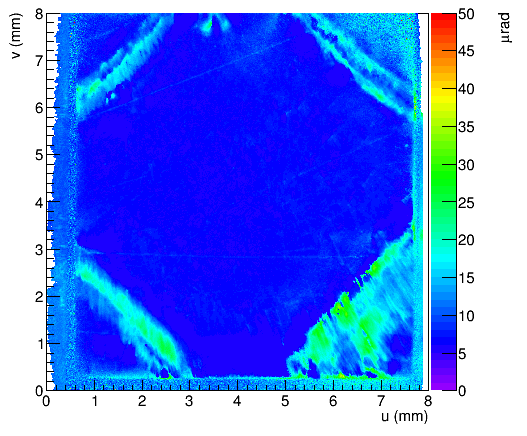
\includegraphics[clip=true,width=0.7\linewidth]{figures/JD70-8-study1_4_sigma_cropped.png}
\end{center}
\caption{(color online) Rocking curve RMS width topograph taken of the (2,2,0) reflection
from a CVD diamond crystal using 15~keV X-rays on C-line at CHESS.
The bright diagonal lines in the corners
indicate regions of increased local strain, coinciding with growth boundaries radiating
outward from the seed crystal used in the CVD growth process. 
        }
\label{fig:diamond_rocking_curve_rms} 
\end{figure}

Fig.~\ref{fig:diamond_rocking_curve_rms} shows a rocking curve topograph of a diamond
radiator taken with 15~keV x-rays at the 
Cornell High Energy Synchrotron Source (CHESS) synchrotron light source. The instrumental
resolution of this measurement is on the same order as the Darwin width for this
diffraction peak, approximately 5 $\mu$rad. During operation, the electron beam spot would
be confined to the relatively uniform central region. Any region in
this figure with a rocking curve root-mean-square width of 20~$\mu$rad or less is indistinguishable
from a perfect crystal for the purposes of \GX{}.
Regardless of whether or not better HPHT diamonds exist, the fact that these Element Six
CVD diamonds have sufficiently narrow diffraction widths for our application, coupled with
their lower cost relative to HPHT material, made them the
obvious choice for the Hall D photon source.

The diamond radiator fabrication procedure began with procurement of the raw
material in the form of $7\times 7\times 1.2$~mm$^3$ CVD single-crystal plates from the
vendor. After x-ray rocking curve scans of the raw material were taken to verify crystal
quality, the acceptable diamonds were shipped to a second vendor, Delaware Diamond Knives (DDK). At DDK, the
1.2-mm-thick samples were sliced into three samples of 250 $\mu$m thickness each, then
each one was polished on both sides down to a final thickness close to 50 $\mu$m. The
samples, now of dimensions $7\times 7\times 0.05$~mm$^3$ were fixed to a small aluminum
mounting tab using a tiny dot of conductive epoxy placed in one corner.
These crystals were then returned to the synchrotron light source
for final x-ray rocking curve measurements prior to final
approval for use in the \GX{} photon source.

The useful lifetime of a diamond radiator in the \GX{} beamline is limited by the 
degradation in the sharpness of the coherent edge due to accumulation of radiation damage.
Experience during the early phase of \GX{} running showed that after exposure to
about 0.5 C of integrated electron beam charge, the width of the coherent edge 
increased enough that the entire coherent peak was no longer contained within the energy
window of the tagger microscope. When a crystal reached that degree of degradation, that
radiator was regarded as no longer usable, and a new crystal was installed.

During Phase 1 of \GX{}, radiator crystals were replaced three times due
to degradation, twice with 50~$\mu$m radiators and once with a 20~$\mu$m. The 20-$\mu$m
diamond was introduced to test if the reduced multiple Coulomb scattering 
might result in an
observable increase in peak polarization. This turned out not to be the case, for
two reasons. The first is that, to take full advantage of the reduced multiple
scattering in the radiator for increased peak polarization, the collimator size 
must be reduced proportionally. A 3.4-mm-diameter collimator was available for
this purpose, but variability observed in the convergence properties of the electron
beam at the radiator overruled running with any collimator smaller than 5~mm,
even when a thinner radiator was in use.

The second reason is that any improvements
from reduced multiple scattering that came with the smaller radiator thickness
were more than offset by strong indications of radiation
damage that appeared not long after the 20~$\mu$m crystal was put into production.
The rapid appearance of radiation damage 
was partly due to the larger beam current (factor 2.5) that was needed to
produce the same photon flux as with a 50~$\mu$m crystal, but that factor alone
did not fully
explain what was seen. Subsequent x-ray measurements showed that a large buckling of
the 20~$\mu$m crystal had occurred in the region of the incident electron beam spot, 
evidently due to  local differential expansion of the diamond lattice arising from
radiation damage. Once the crystal buckled, the energy of the coherent
peak varied significantly across the electron beam spot, effectively broadening
the peak. Fortunately, the greater stiffness of a 50~$\mu$m crystal
appears to suppress this local buckling under similar conditions of radiation damage.

Based on these observations, 50~$\mu$m was selected as the
optimum thickness for \GX{} diamond radiators: thin enough to limit the effects
of multiple scattering and thick enough to suppress buckling from internal stress
induced by radiation damage. The effective useful lifetime of a 50~$\mu$m radiator
in the photon source is about 0.5 C integrated incident electron charge. 
This lifetime might be extended somewhat by the use of thermal annealing to partially remove the effects of radiation damage. As the pace of diamond replacement increases with the start of \GX{} Phase 2 full-intensity running and the number of spent radiators
starts to accumulate, this possibility will be explored.

\begin{figure}[tbp]
\begin{center}
   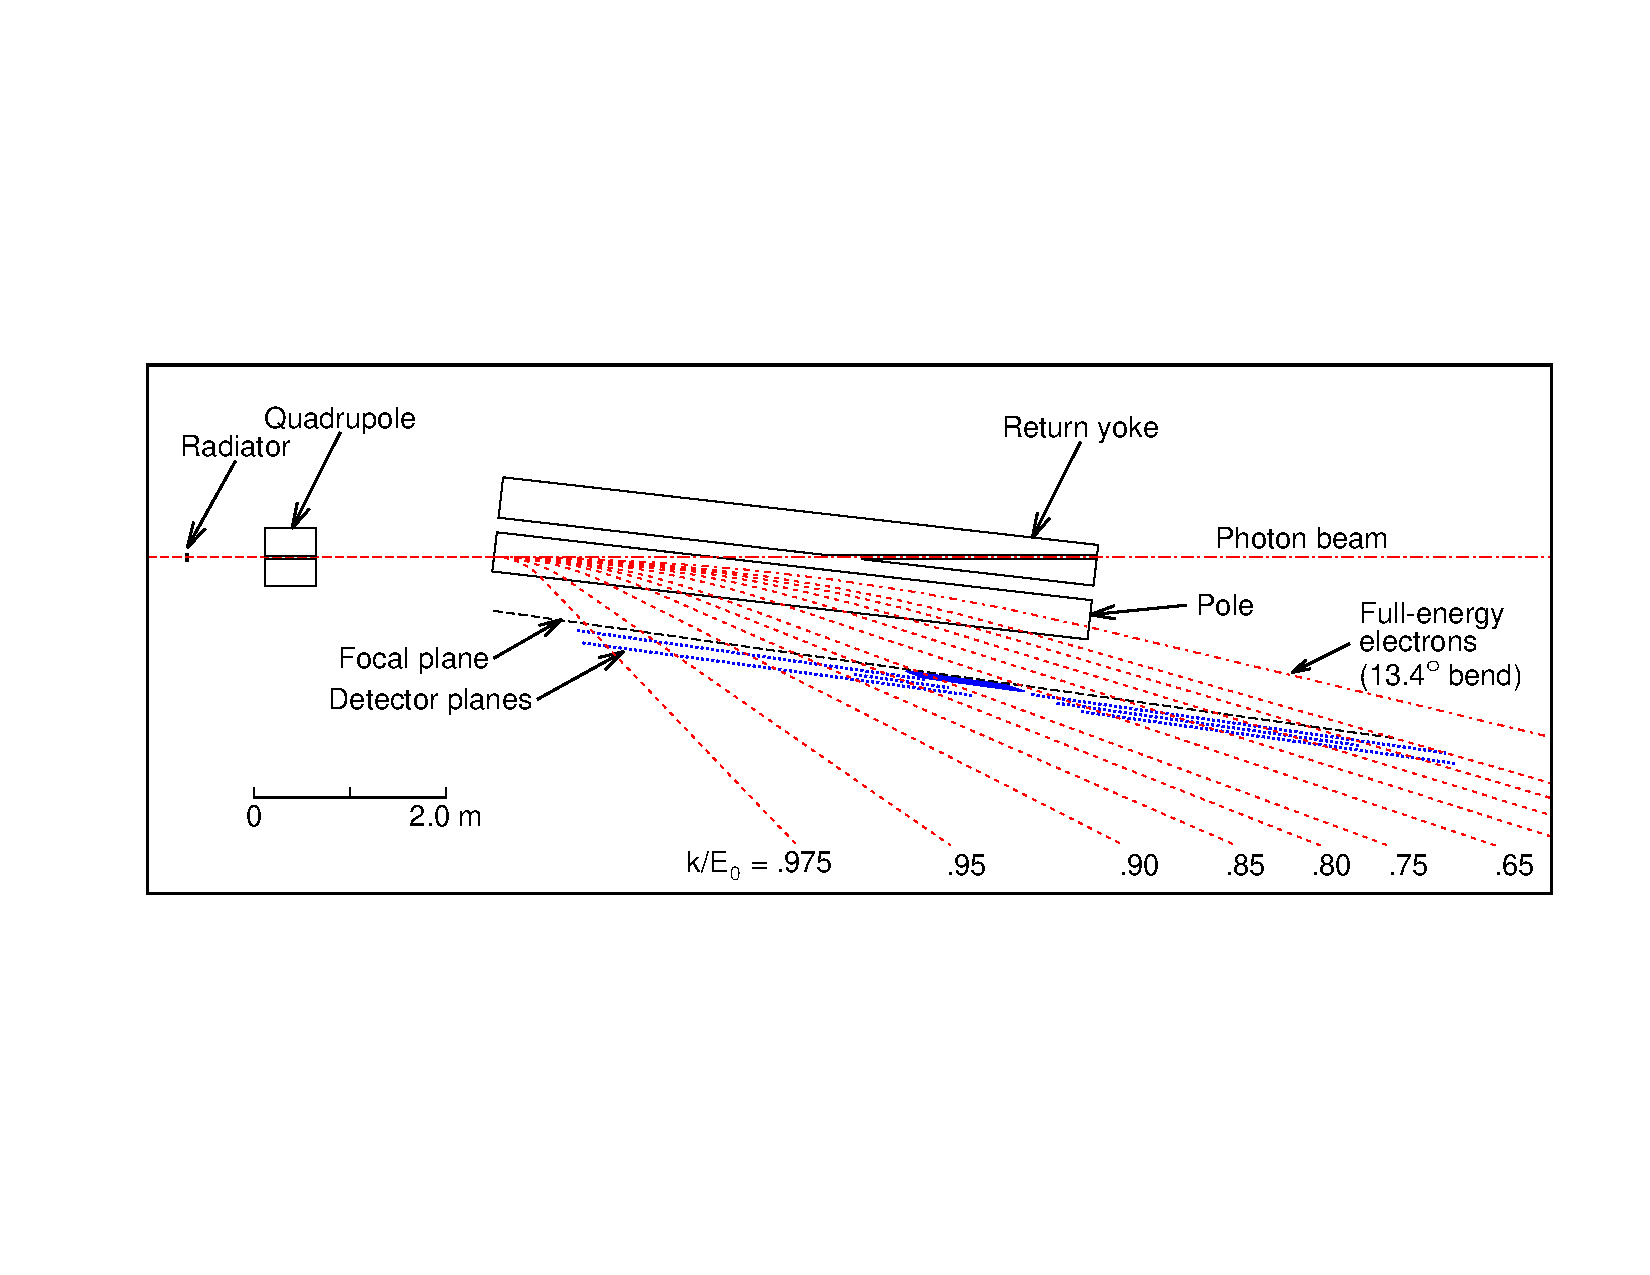
\includegraphics[width=0.95\linewidth,viewport=80 200 750 400]{figures/BEAM_taggerplot.pdf}
%   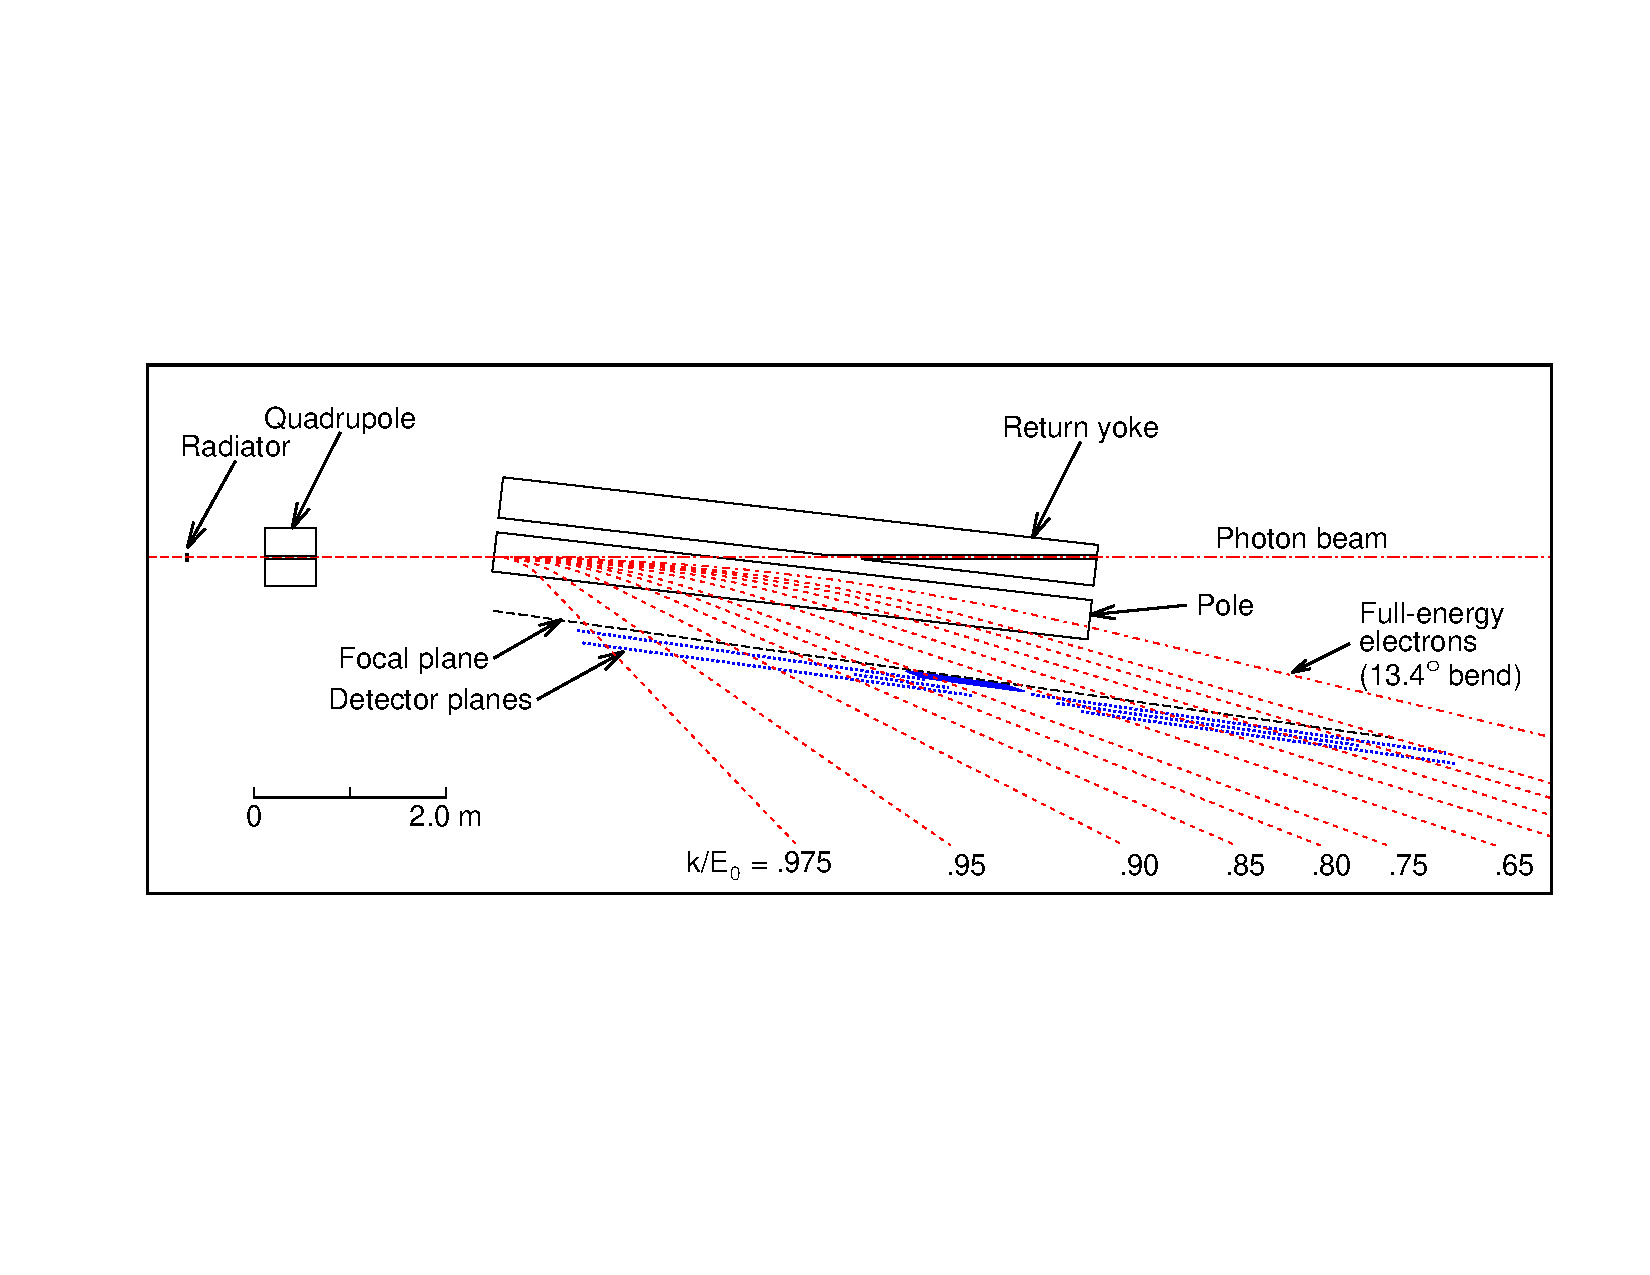
\includegraphics[width=0.95\linewidth,viewport=150 115 628 500]{figures/BEAM_taggerplot.pdf}
%      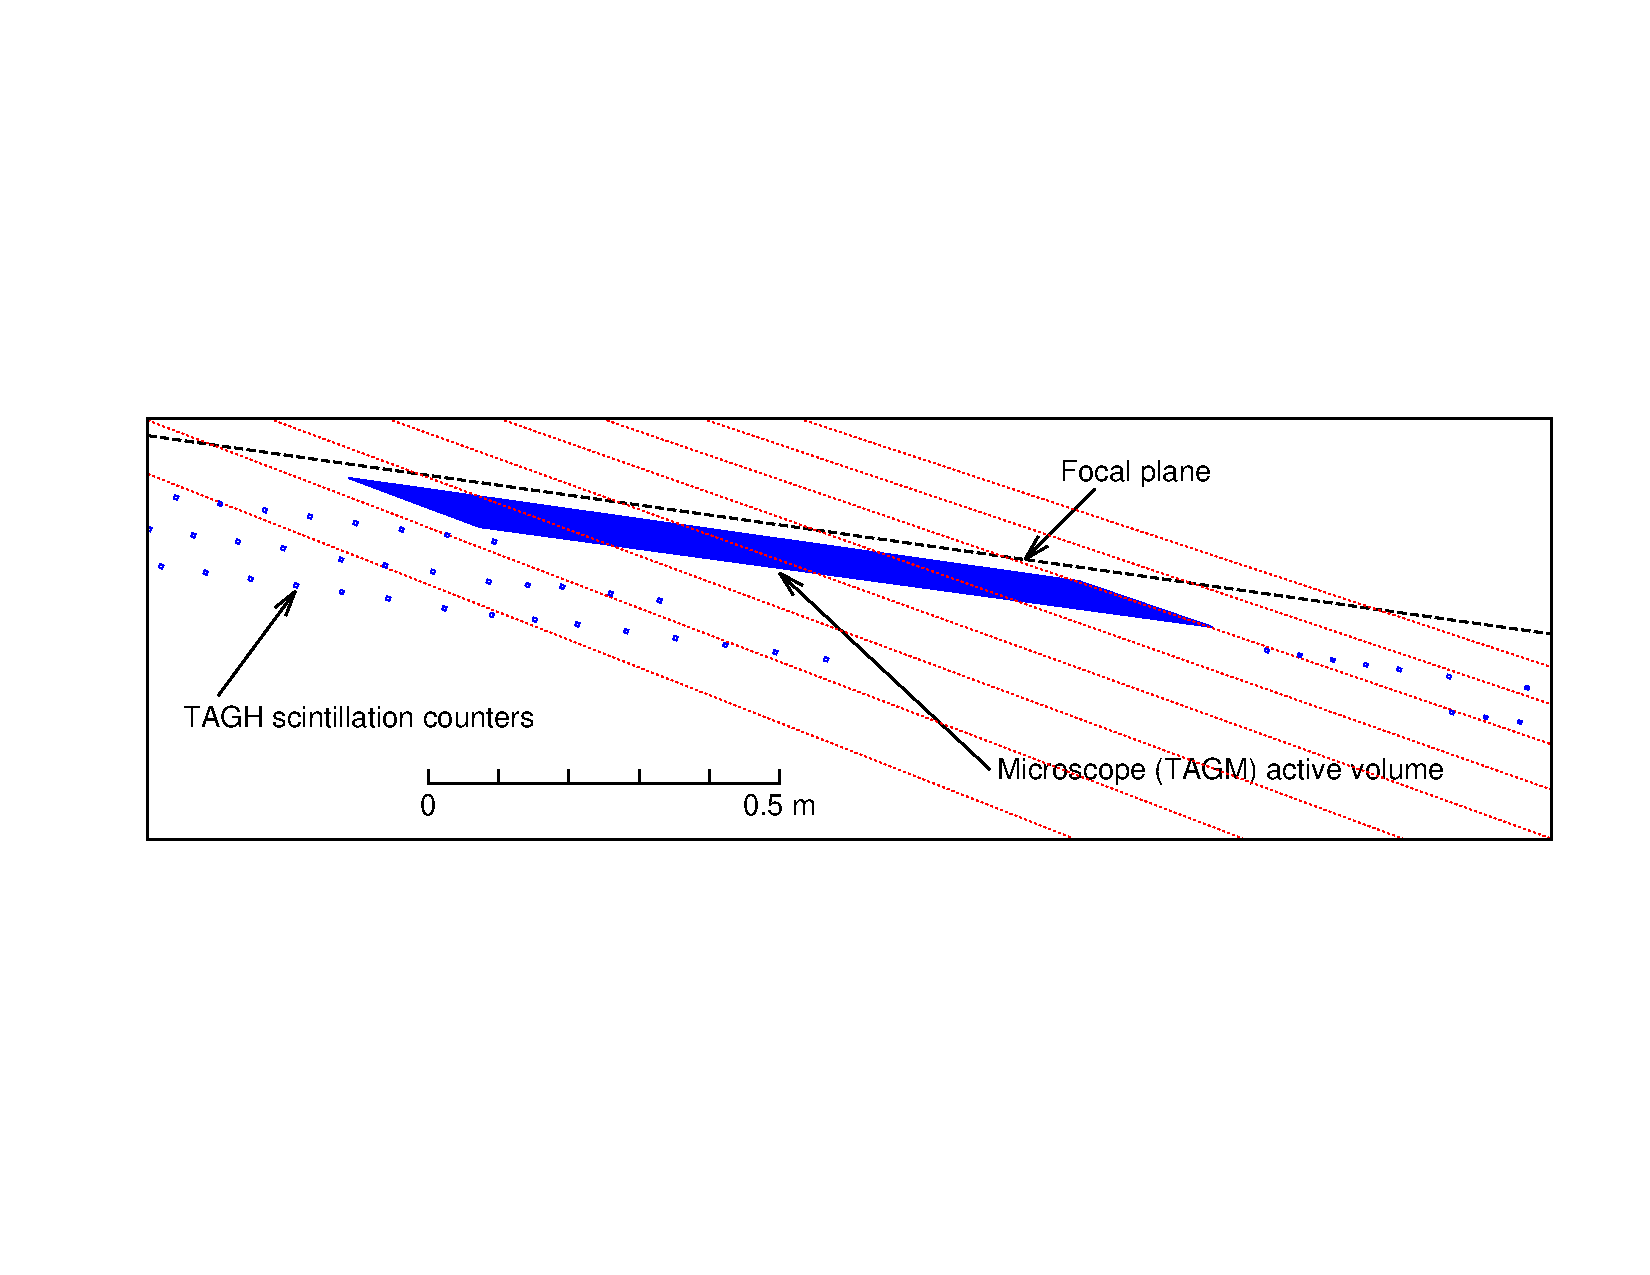
\includegraphics[width=0.95\linewidth]{figures/BEAM_taggerdetectors.pdf}
\caption{Schematic diagram of the tagging spectrometer, showing the paths of the electron
and photon beams. Dotted lines indicate post-radiation electron trajectories identified by
the energy the electron gave up to an associated radiated photon, as a fraction of the beam energy E$_0$.
The tagger focal plane detector arrays TAGH and TAGM are described in the text.
       \label{fig:beam:BEAM_taggerplot}  }
\end{center}
\end{figure}

\subsection{Photon tagging system \label{sec:tag}}
After passing through the radiator, the combined photon and electron beams enter
the photon tagging spectrometer (``tagger''), where the full-energy electrons are swept out of
the beamline by a dipole magnet and redirected into a shielded beam dump. The
subset of beam electrons that radiated a significant fraction of their energy in
the radiator are bent further in the dipole field. 
These post-brems\-strah\-lung electrons exit through a thin window
along the side of the magnet, where these
electrons are intercepted by a highly segmented
array of scintillators called the tagger hodoscope (TAGH), as shown in
Fig.\,\ref{fig:beam:BEAM_taggerplot}. In addition to the TAGH counters that span
the full range in energy from 25\% to 97\% of the full electron beam energy, a high-energy-resolution device known as the tagger microscope (TAGM) covers the
energy range corresponding to the primary coherent peak, indicated by the denser
portion of the focal plane in Fig.\,\ref{fig:beam:BEAM_taggerplot}. 
The quadrupole magnet upstream of the tagger dipole provides a weak vertical focus
to optimize the efficiency of the tagger microscope for tagging collimated photons.
Downstream of the tagger magnet
on the photon beam line, a 0.8~T$\cdot$m permanent dipole magnet is installed to prevent the electron beam from reaching
Hall D should the tagger magnet trip.

Both the TAGM and TAGH devices are used to determine the energy of individual
photons in the photon beam via coincidence, using
the relation $E_{\gamma} = E_{0} - E_{e}$, where $E_{0}$ is the primary electron
beam energy before interaction with the radiator, and $E_{e}$ is the
energy of the post-brems\-strah\-lung electron determined by its detected position at the
focal plane. Multiple radiative interactions in a 50 $\mu$m diamond radiator
($3\times 10^{-4}$ radiation lengths) produce uncertainty in the value of
$E_{\gamma}$ of the same order as the intrinsic energy spread of the incident
electron beam.

\subsubsection{Tagger magnet \label{sec:tagMagnet}}
The Hall D tagger magnet deflects electrons in the horizontal plane, allowing the
brems\-strah\-lung-produced photons to continue to the experimental hall while
bending the electrons that produced them into the focal plane detectors.
Electrons that lost little or no energy in the
radiator are deflected by 13.4$^\circ$ into the electron beam dump.

The Hall D tagger magnet is an Elbek-type room temperature dipole magnet, similar
to the JLab Hall B tagger magnet \cite{BORGGREEN19631, Sober2000263}. 
The magnet is 1.13 m wide, 1.41 m high and 6.3 m long, weighing 80 metric tons,
with a normal operating field of 1.5 T for a  12 GeV incident electron beam, 
a maximum field of 1.75 T, and a pole gap of 30 mm. 
The magnet
design was optimized using the detailed magnetic field calculation  provided by the
TOSCA simulation package and the ray tracing of electron beam trajectories~\cite{DIPOLE_YANG,DIPOLE_SOMOV}.

The GlueX experiment requires that the scattered
electron beam be measured with an accuracy of 12~MeV (0.1\% of the incident electron
energy). This requires that the magnetic field integrals along all useful electron
trajectories be known to 0.1\%. The magnetic field was mapped at Jefferson Lab and
the detailed field maps were augmented by detailed TOSCA calculations which have
allowed us to meet these goals. Details of the magnet mapping and uniformity are
found in Ref.\,\cite{gx4271}.

\subsubsection{Tagger microscope}\label{sec:TAGM}
The tagger microscope (TAGM) is a high-resolution hodoscope that counts post-~\!\!brems\-strah\-lung electrons corresponding to the primary coherent peak.
Normally the TAGM is positioned to cover between 8.2 and 9.2~GeV in photon energy, but TAGM is designed to be movable should a different peak energy be desired.
The microscope is segmented along the horizontal axis into 102 energy bins (columns) of approximately equal width. Each column is segmented 
in 5 sections (rows) along the vertical axis, for a total of 510 independent electronic
channels. The vertical segmentation allows the possibility of scattered electron
collimation, which gives a significant increase in photon polarization when used in
combination with photon collimation. The purpose of the quadrupole magnet upstream
of the dipole is to provide the vertical focus needed to make the
double-collimation scheme work efficiently. Summed signals are also available for
each column for use in normal operation when electron collimation is not desired.

The tagger microscope consists of a two-dimensional array of square scintillating
fibers packed in a dense array of dimensions $102\times 5$. The fibers are multi-clad
BCF-20 with a $2\times 2$ mm$^2$ square transverse profile, manufactured by Saint Gobain.
The cladding varies in thickness from 100 microns near the corners to 70 microns in
the middle of the sides, with an active area of $1.8\times 1.8$~mm$^2$ per fiber.
Variations at the level of 5\% in the transverse size of the fibers impose a practical
lower bound of 2.05~mm on the pitch of the array. The detection efficiency of the TAGM
averages 75\% across its full energy range, in good agreement with the geometric
factor of 77\%.

Each scintillating fiber is 10~mm long, fused at its downstream end to
a clear light guide of matching dimensions (Saint Gobain BCF-98) that
transmits the scintillation light away from the focal plane to a shielded box where
a silicon photomultipliers (SiPM) converts light pulses into electronic signals. The
scintillators are oriented so that the electron trajectories are parallel to the
fiber axis, providing large signals for electrons from the radiator, in contrast
to the omni-directional electromagnetic background that fills the tagger hall.

\begin{figure}[tbh]
\begin{center}
 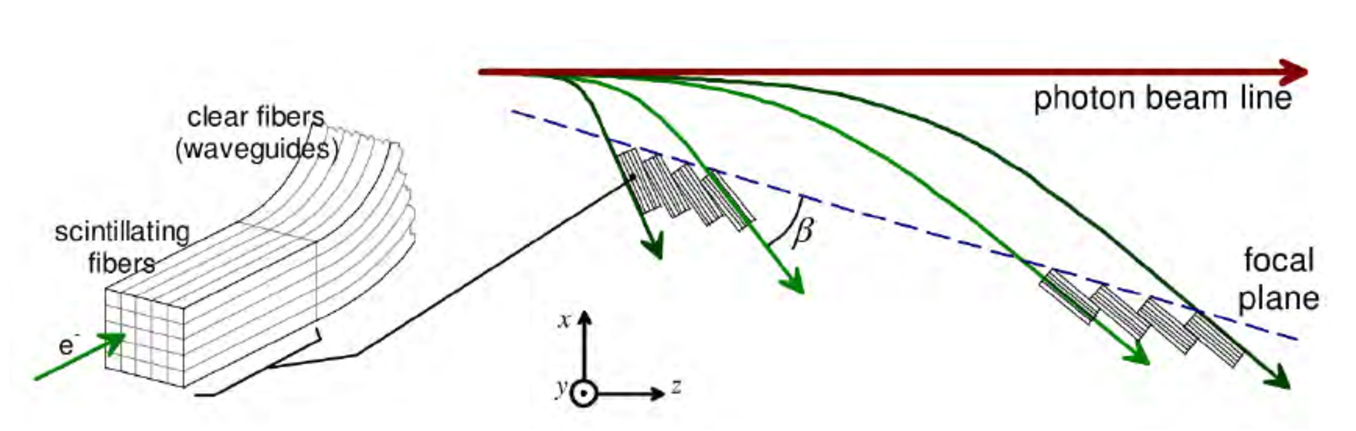
\includegraphics[clip=true,width=0.95\linewidth]{figures/TAGM_conceptual.pdf}
\end{center}
\caption{
Conceptual overview of the tagger microscope design, showing the fiber bundles and
light guides (left), and the orientation of these bundles aligned with the incoming
electron beam direction in the tagger focal plane (right). The variation of the
crossing angle $\beta$ is exaggerated for sake of illustration.
        }
\label{fig:TAGM_conceptual}
\end{figure}

Because the electron trajectories do not cross the focal plane at right angles, the
fiber array must be staggered along the dispersion direction. A staggering step
occcurs every 6 columns, as illustrated in Fig.~\ref{fig:TAGM_conceptual}. The slight
variation of the crossing angle $\beta$ is taken into account by a carefully adjusted
fan-out that is implemented by small evenly-distributed gaps at the rear ends of 
adjacent 6-column groups (bundles). A total of 17 such bundles comprise the full
tagger microscope.

The far ends of the scintillation light guides are coupled to Hamamatsu S10931-050P SiPMs. The SiPMs are mounted on a custom-built two-stage preamplifier board, with 15 SiPMs per board. In addition to the 15 individual signals generated
by each preamplifier, the boards also produce three analog sum outputs, each the sum
of five adjacent SiPMs corresponding to the five fibers in a single column. All 510
SiPMs are individually biased by custom bias control boards, one for every two
preamplifier boards. The control boards connect to the
preamplifiers over a custom backplane, and communicate with the
experimental slow controls over ethernet. Each control board has the
capability to electronically select between two gain modes for the preamplifiers
on that board:
a low gain mode used during regular tagging operation, and a high gain
mode used for triggering on single-pixel pulses during bias calibration.
Each bias control board manages the control and biasing for two preamplifiers.
The control board also measures live values for environmental parameters
(voltage levels and temperatures) in the TAGM electronics, so that alarms can
be generated by the experimental control system whenever any of these parameters
strays outside predefined limits.

Pulse height and timing information for 122 channels from the TAGM is provided by analog-to-digital converters (ADCs) and time-to-digital converters (TDCs). These 122
signals include the 102 column sums plus the individual fiber signals from
columns 7, 27, 81, and 97. Each signal for these 122 channels goes through a 1:1
passive splitter, with one output going to an ADC and the other through
discriminators to a TDC. The ADCs are 250-MHz flash ADC's with 12-bit
resolution and a full-scale pulse amplitude of 1 V. The TDCs are based
on the F1TDC chip, with a least-count of 62~ps. Pulse thresholds in both
the ADC and discriminator modules are programmable over the range 1-1000 mV
on an individual channel basis, covering the full dynamic range of the TAGM
frontend. The TAGM preamplifier outputs (before splitting) saturate around
2~V pulse amplitude.

The mean pulse charge in units of SiPM pixels corresponding to a
single high-energy electron varies from 150 to 300 pC, depending on the fiber,
with an average of 220 pC and standard deviation of 25 pC. During calibration,
this yield is measured individually for each fiber by selectively biasing
the SiPMs on each row of fibers, one row at a time, and reading out the column
sums. Once all 510 individual fiber yields have been measured, the bias voltages
within each column are adjusted to compensate for yield variations, so
that the mean pulse height in a given column is the same regardless of which
fiber in the column detected the electron. The ADC readout and discriminator
thresholds are set individually for each column, for optimum efficiency and
noise rejection.

The ADC firmware provides an approximate time for each pulse, in addition to the
pulse amplitude. During offline reconstruction, this time information is used to
associate ADC and TDC pulse information from the same channel, so that a
time-walk correction can be applied to the TDC time. Once this correction
has been applied, a time resolution of 230~ps is achieved for the TAGM.
This resolution is based on data collected at rates on the order of 1~MHz
per column, a factor of 2 lower than the 2.2~MHz peak rate anticipated during
\GX{} Phase 2 running. A brief test above 2~MHz per column allowed visual
inspection of the pulse waveforms from the TAGM, and no change in the
pulse shape or amplitude was observed. Given that the readout was designed
to operate at rates up to 4~MHz per column without significant degradation
in performance, the TAGM time resolution should be
substantially unaffected by the increased beam intensity of \GX{} Phase 2.

\subsubsection{Broadband tagging hodoscope}\label{sec:TAGHIntro}
The tagger hodoscope (TAGH) is a device consisting of $\sim$220 scintillator counters distributed over a length of 9.25~m and mounted just behind the focal plane of the tagger magnet.
The function of this hodoscope is to tag the full range in photon energy from 25\% to 97\%
of the incident electron energy, with a gap in the middle of that range
left open for the tagger microscope. The geometry of the counters in the
vicinity of the microscope is shown in Fig.\,\ref{fig:beam:BEAM_taggerdetectors}. 
This broad coverage aids in alignment of the diamond radiator and expands the \GX{} physics program reach to photon energies outside the range of the coherent peak.
The coverage of the hodoscope counters in the region below 60\% drops to half,
with substantial gaps in energy between the counters. This was done because
the events of primary interest to \GX{} come from interactions of photons
within and above the coherent peak; 
within and above the coherent peak the coverage is 100\% up to the 97\% $E_0$ cutoff.

Each counter in the hodoscope is a sheet of EJ-228 scintillator, 6 mm thick and
40 mm high. The counter widths vary along the focal plane, from 21~mm near the
end-point region down to 3~mm at the downstream end. The scintillators are
coupled to a Hamamatsu R9800 photomultiplier tube (PMT) via a cylindrical acrylic (UVT-PMMA) light
guide 22.2 mm in diameter and 120 mm long. Each PMT is wrapped in $\mu$-metal
to shield the tube from the fringe field of the tagger magnet.

Each PMT is instrumented with a locally-designed active base~\cite{tagh:base},
consisting of a high-voltage divider and an amplifier powered by current
flowing through the divider. The base provides two signal outputs, one going
to a flash ADC and the other through a discriminator to a TDC.
Operating the amplifier with a gain factor of 8.5 allows the PMT to operate at a
lower voltage of 900 V and reduce the PMT anode current, therefore improving
the rate capability. The energy bite of each counter ranges between 8.5 and
30 MeV for a 12 GeV incident electron beam.  Typical rates during production
running are 1 MHz above the coherent peak and 2 MHz per counter below the
coherent peak. The maximum sustainable rate per counter is about 4~MHz.

The counters are mounted with their faces normal to the path of the
scattered electrons in two or three rows slightly downstream of the focal
plane, as shown in Fig.\,\ref{fig:beam:BEAM_taggerdetectors}.
This mounting approach allows the counters to be positioned without horizontal gaps in
the dispersion direction, enabling complete coverage of the entire
tagged photon energy range.

\begin{figure}[tbp]
\begin{center}
%   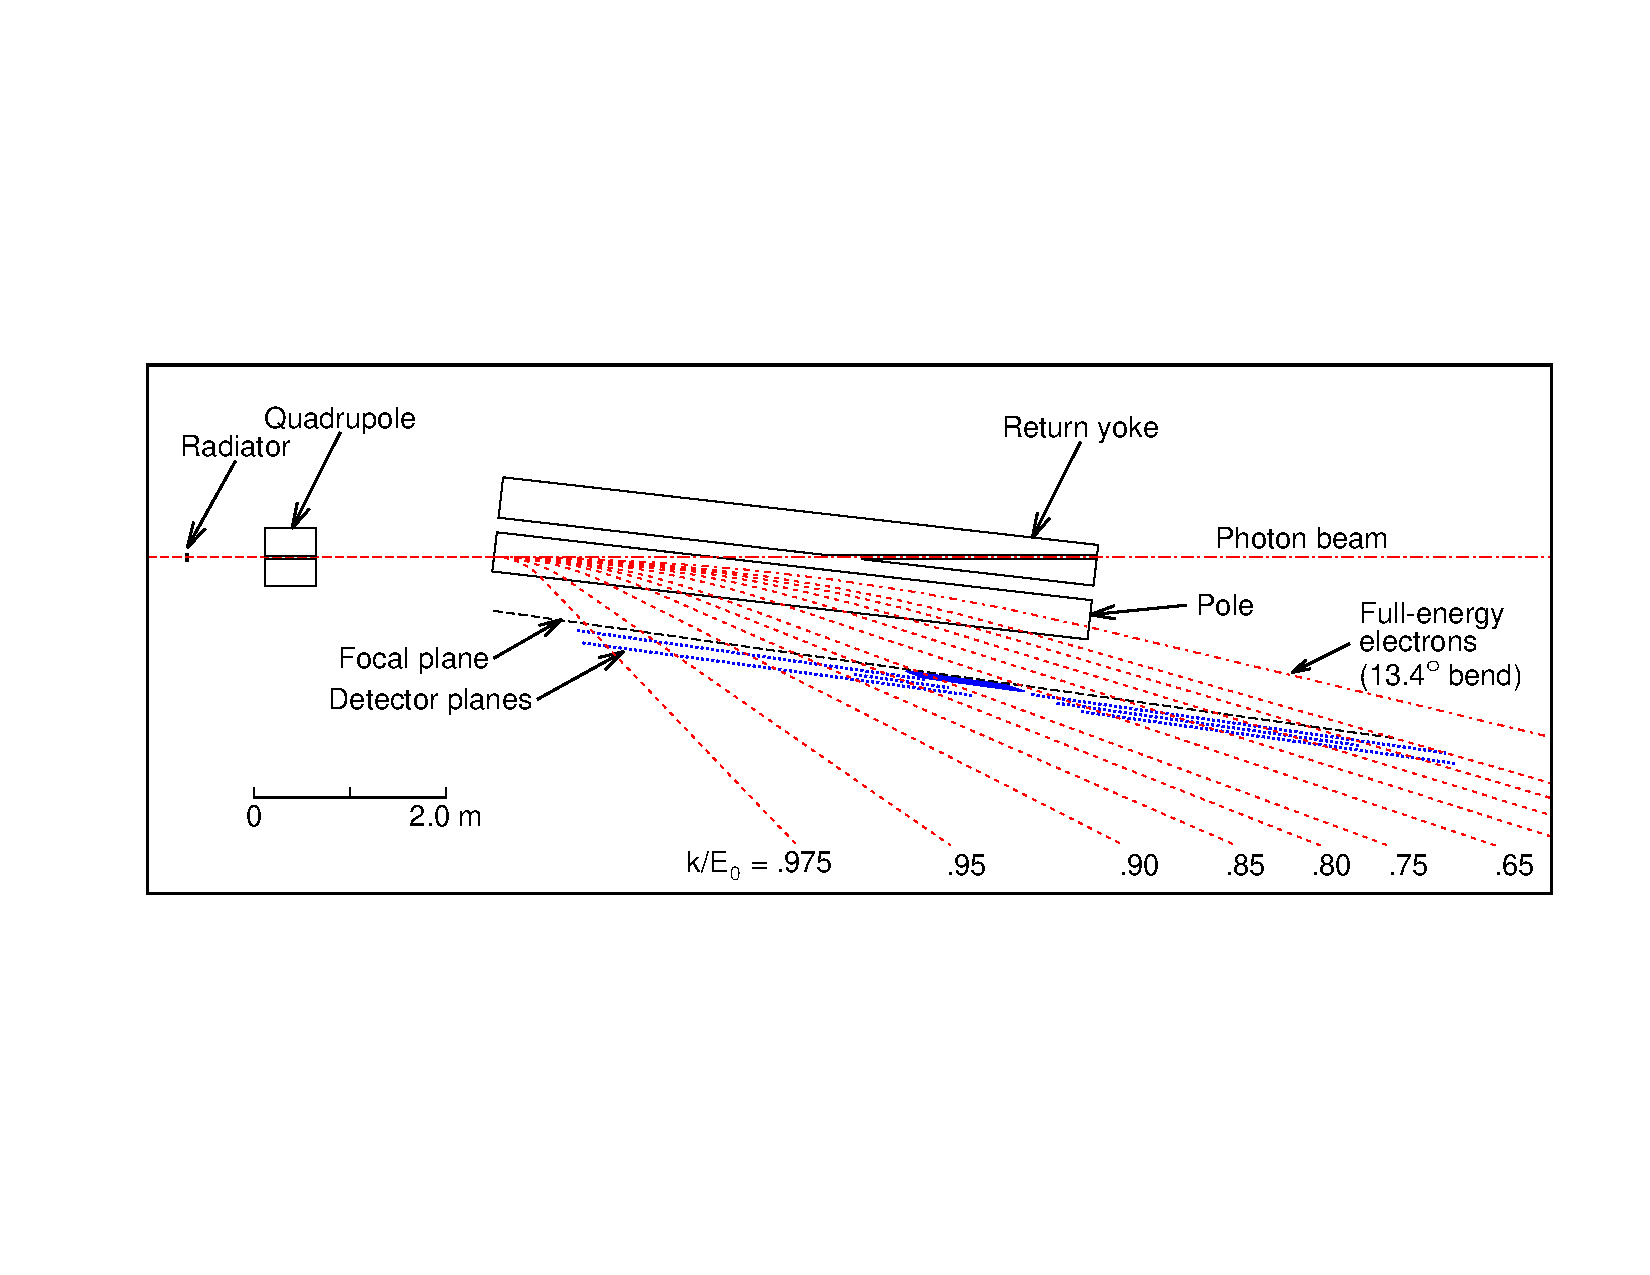
\includegraphics[width=0.95\linewidth]{figures/BEAM_taggerplot.pdf}
%   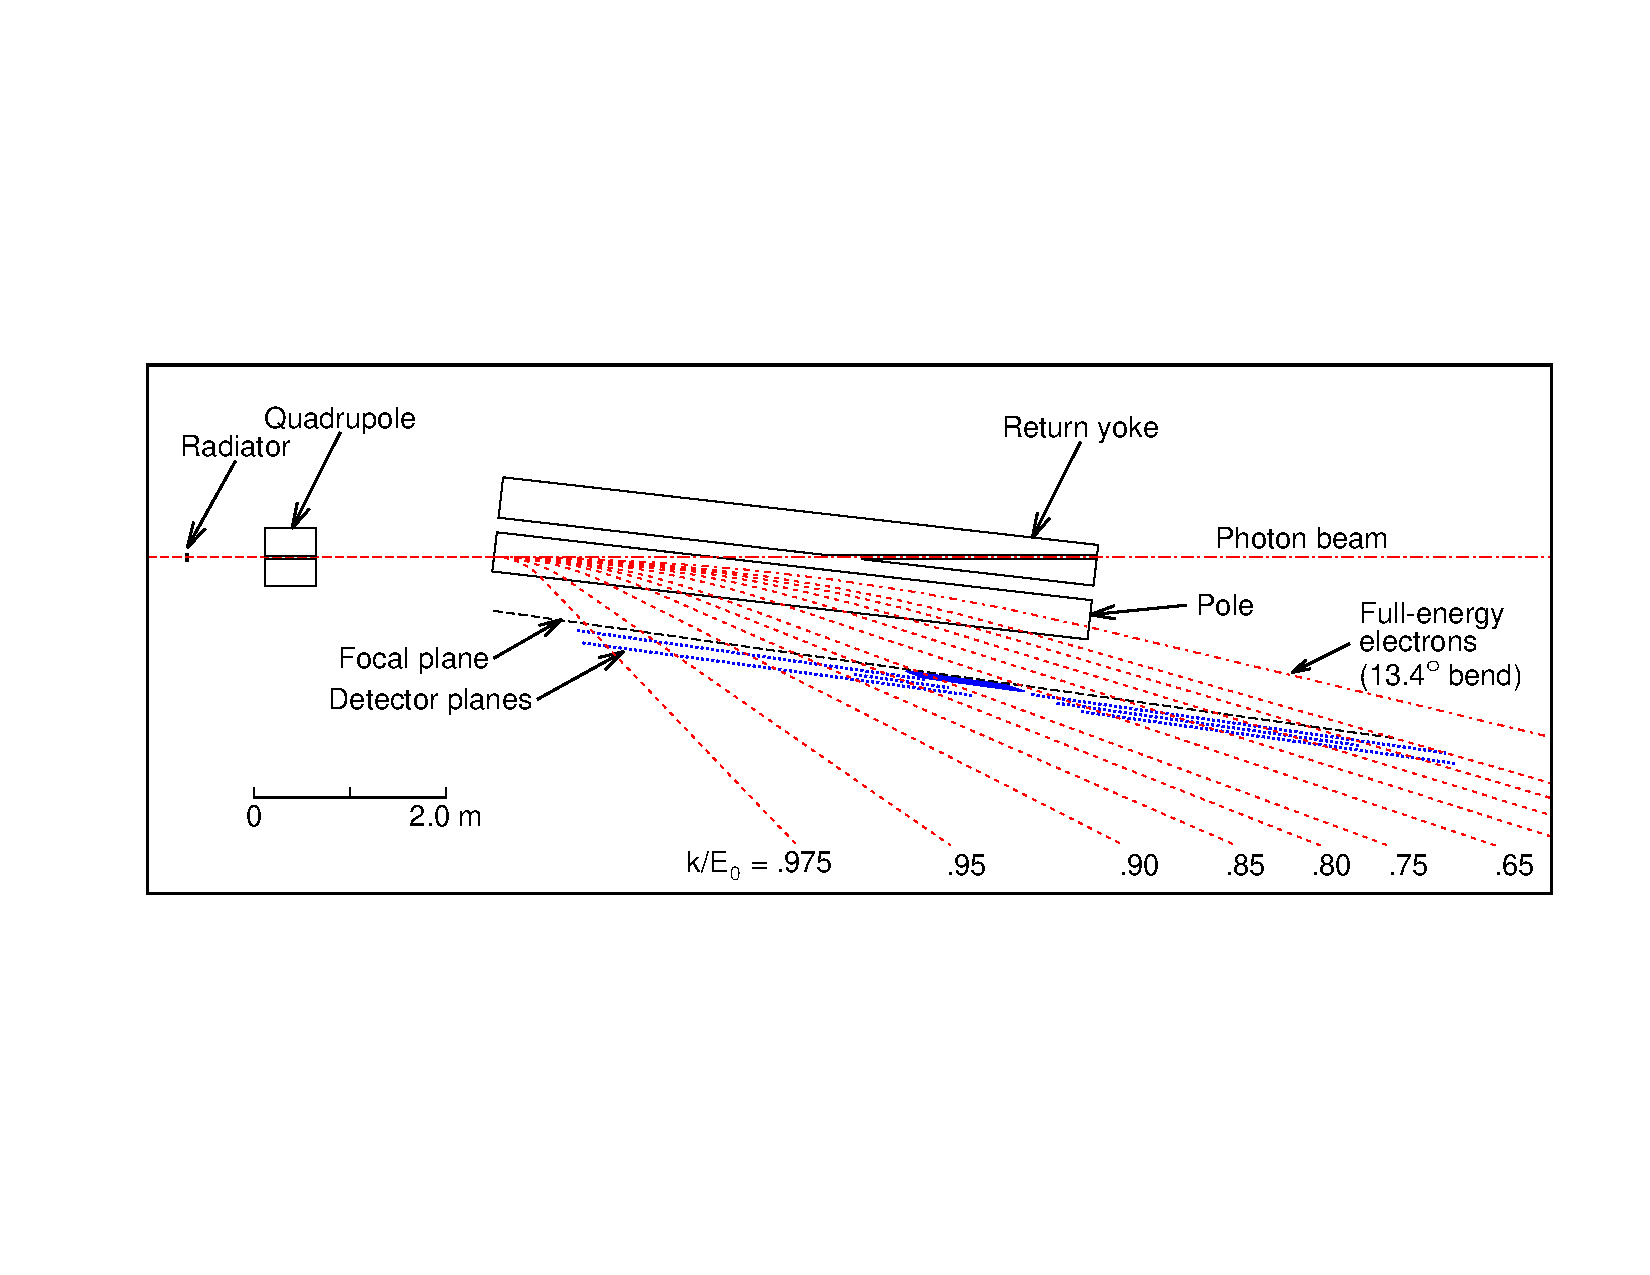
\includegraphics[width=0.95\linewidth,viewport=150 115 628 500]{figures/BEAM_taggerplot.pdf}
      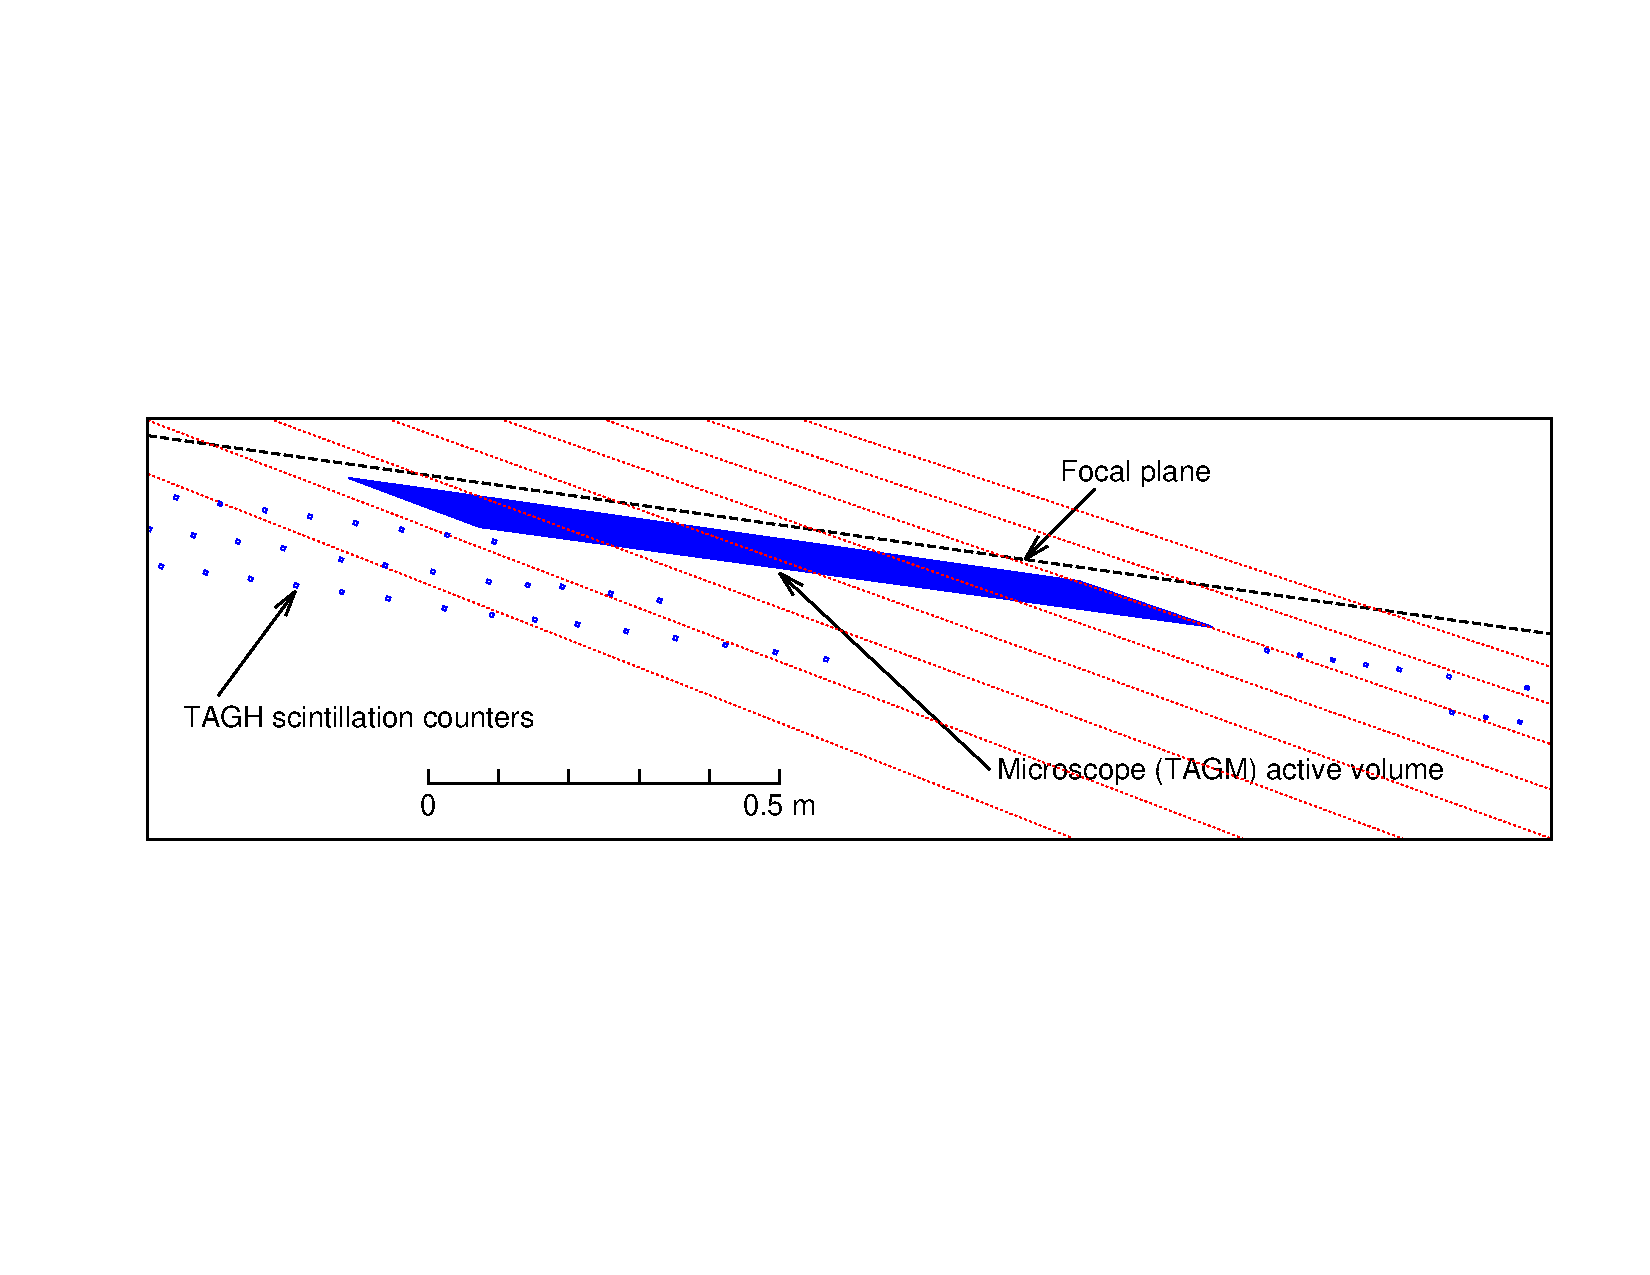
\includegraphics[width=0.95\linewidth,viewport=80 200 750 400]{figures/BEAM_taggerdetectors.pdf}
\caption{Schematic of electron trajectories in the region of the microscope. Shown are the three layers of hodoscope counters on either side of the microscope and the 
               region covered by the microscope.
       \label{fig:beam:BEAM_taggerdetectors}  }

\end{center}
\end{figure}

The mounting frame of the hodoscope is suspended from the ceiling of the Tagger Hall
to provide full flexibility for positioning TAGH. The frame is constructed
to also support the addition of counters to fill in the energy range currently
occupied by the microscope when the TAGM location is changed.

A similar procedure to that described above for the TAGM is used to apply
a time-walk correction to the TDC times from the TAGH counters. Once this
time-walk correction
is applied, the time resolution of the TAGH is 200~ps. No significant
degradation of this resolution is expected at the operating rates planned
for Phase 2 running, which are on the order of 2 MHz per counter above
the coherent peak. Under these conditions, the rates in the TAGH counters
below the coherent peak would average around 4~Mhz, which is at the top
of their allowed range; these counters will normally be turned off when
running at full intensity in Phase 2.

\subsection{Beam profiler}
The beam profiler is located immediately upstream of the collimator and is
used to measure the photon beam intensity in a plane normal to the incident
photon beam. The profiler consists of two planes
of scintillating fibers, giving information on the photon beam profile
in the X and Y projections. Each plane consists of 64 square fibers,
2 mm in width, read out by four 16-channel multi-anode PMTs. The beam profiler
is only used during beam setup until the photon beam is centered on the active collimator.
This beam profiler can be used reliably to provide feedback on
the beam position during setup, but is retracted during physics production runs.

\subsection{Active collimator \label{sec:coll}}
The active collimator monitors the photon beam position and provides
feedback to micro-steering magnets in the electron beamline, for the
purpose of suppressing drifts in photon beam position. 
The
design of the active collimator for \GX{} is based on a device 
developed at SLAC for monitoring
the coherent bremsstrahlung beam there \cite{Miller:1973yi}.
The \GX{} active collimator is located on
the upstream face of the primary collimator, and consists of a dense
array of tungsten pins attached to tungsten base plates. The tungsten
plate intercepts off-axis beam photons before they enter the collimator,
creating an electromagnetic shower that cascades through the array
of pins. High-energy delta rays created by the
shower in the pins (known as ``knock-ons") 
are emitted forward into the primary collimator, and
result in a net current between the tungsten plates and the collimator
that is proportional to the intensity of the photon beam on the plate.
The tungsten plates are mounted on an insulating support, and the plate
currents are monitored by a preamplifier with pA sensitivity. 

The tungsten plate is segmented radially into two rings, and each ring is
segmented azimuthally into four quadrants. The asymmetry of the induced 
currents on the plates in opposite quadrants indicate the degree of
displacement of the photon beam from the intended center position. Typical
currents on the tungsten sectors are at the level of 1.4~nA (inner ring)
and 0.85~nA (outer ring) when running with a 50~$\mu$m diamond crystal
and a 200-nA incident electron beam current. The current-sensitive preamplifiers
used with the active collimator are PMT-5R devices manufactured by
ARI Corporation. The PMT-5R has six remotely selectable gain settings
ranging from $10^{12}$~V/A to $10^6$~V/A, selectable by powers of 10.
This provides excellent dynamic
range for operation of the beam over a wide range of intensities, from
1~nA up to several $\mu$A. The preamplifier input stage exhibits a fixed
gain-bandwidth product of about 2~Hz-V/pA which limits its bandwidth at
the higher gain settings, for example 2~Hz at $10^{12}$~V/A, 20~Hz at
$10^{11}$~V/A, and so on.

In-situ electronic noise on the individual wedge currents is measured to
be 1.5~pA/$\sqrt{\mbox{Hz}}$ on the inner ring, and 15~pA/$\sqrt{\mbox{Hz}}$
on the outer ring. The sensitivity of the current asymmetry to position is
0.160/mm for the inner ring and 0.089/mm for the outer. The electronic
noise on the individual wedge currents is 1.5~pA/$\sqrt{\mbox{Hz}}$
(inner ring) and 15~pA/$\sqrt{\mbox{Hz}}$ (outer ring).
With a 50~micron diamond and 200~nA beam current, operating the active
collimator at a bandwidth of 1~kHz yields a measurement error in the
position of the beam centroid of 150~$\mu$m for the inner ring and
450~$\mu$m for the outer ring.
The purpose of the outer ring is to help locate the beam when the beam location
has shifted more than 2~mm from the collimator axis, where the response
of the inner ring sectors becomes nonlinear.

The maximum deviation allowed for the Hall D photon beam position 
relative to the collimator axis is 200~$\mu$m. The active collimator
readout was designed with kHz bandwidth so that use in a
fast feedback loop would suppress motion of the beam at 60~Hz and harmonics
that might exceed this limit. Experience with the Hall D beam has shown
that the electron beam feedback systems already suppresses this motion
to less than 100~$\mu$m amplitude, so that fast feedback using the active
collimator is not required during normal operation. Instead, the active collimator is
used in a slow feedback loop which locks the photon beam position at
the collimator with a correction time constant of a few seconds. This
slow feedback system
is essential for preventing long-term drifts in the photon beam
position that would otherwise occur on the time scale of hours or
days. Operating in this mode with noise averaging over 5 s intervals,
the  active collimator can achieve 200~$\mu$m position resolution down
to beam currents as low as 2~nA. 

\subsection{Collimator}
The photon beam produced at the diamond radiator contains both incoherent
and coherent bremsstrahlung components. In the region of the coherent peak,
where photon polarization is at its maximum, the angular spread of coherent
bremsstrahlung photons is less than that of incoherent bremsstrahlung.
The characteristic emission angle for incoherent bremsstrahlung is
$m/E = 43$~$\mu$rad at 12~GeV, whereas the coherent flux within the
primary peak is concentrated below 15~$\mu$rad with respect to the beam
direction. Collimation increases the degree of linear polarization in
the photon beam by suppressing the incoherent component relative to the
coherent part.

The Hall D primary collimator provides apertures of 3.4 mm and 5.0 mm in a
tungsten block mounted on an X-Y table. The 5.0~mm collimator is used
Under normal \GX{} running conditions.
The tungsten collimator is surrounded by lead shielding.
The collimator may also be positioned to block the beam to prevent
high intensity beam from entering the experimental hall during tuning
of the electron beam. Downstream of the primary collimator, a
sweeping magnet and shield wall, followed by a secondary collimator
with its sweeping magnet and shield wall, suppress charged
particles and gamma background around the photon beam that are
generated in the primary collimator. The photon beam exiting the
collimation system then passes through a thin pair conversion target
that allows continuous monitoring of the photon beam flux and polarization.

\subsection{Triplet polarimeter \label{sec:tpol}}
The triplet polarimeter (TPOL) is used to measure the degree of polarization
of the linearly-polarized photon beam \cite{DUGGER2017115}.
The polarimeter uses the process of $e^+e^-$ pair production on atomic electrons 
in a beryllium target foil, with these scattered atomic electrons
measured using a silicon strip detector.
Information on the degree of polarization of the photon beam is
obtained by analyzing the azimuthal distribution of the scattered
atomic electrons measured by this device.

\subsubsection{Determination of photon polarization \label{sec:polarization}}
Triplet photoproduction occurs when the polarized electron beam interacts
with the electric field of an atomic electron within a target material
and produces a high energy $e^+e^-$ pair. When coupled with
trajectory and energy information of the $e^+e^-$ lepton pair, the azimuthal
angular distribution of the recoil electron provides a measure of
the photon beam polarization. The cross section for triplet photoproduction
can be written as $\sigma_t = \sigma_0 [ 1 - P \Sigma \cos(2\varphi)]$
for a polarized photon beam, where $\sigma_0$ is the unpolarized triplet
cross section, $P$ the photon beam polarization, $\Sigma$ the beam
asymmetry for the process, and $\varphi$ the azimuthal angle of the
recoil electron trajectory with respect to the plane of polarization
for the incident photon beam. To determine the photon beam polarization,
the azimuthal distribution of the recoil electrons is recorded and fit
to the function $A [ 1- B \cos(2\varphi)]$  where the variables $A$ and
$B$ are parameters of the fit, with $B = P \Sigma$. The value of
$\Sigma$ depends on the intensity profile of the photon beam, the
thickness of the converter target, and many other details of the setup.
The value of $\Sigma$ was determined to be $0.1990 \pm 0.0008$ at 9~GeV for the \GX{} beamline
and a 75~micron Be converter~\cite{DUGGER2017115}.

The triplet polarimeter (TPOL) detects the recoil electron arising
from triplet photoproduction. This system consists of a converter tray and
positioning assembly, which holds and positions a beryllium foil converter
within which the triplet photoproduction takes place; a silicon strip detector
(SSD) to detect the recoil electron from triplet photoproduction, providing
energy and azimuthal angle information for that particle; a vacuum housing,
containing the production target and SSD, supplying a vacuum environment
minimizing multiple Coulomb scattering between target and SSD, and lastly
the preamplifier and signal filtering electronics within a Faraday-cage
housing. In the preamp enclosure, to reduce exterior electromagnetic
signal interference, the box is lined with a layer of copper foil.
Signals from the downstream (azimuthal sector) side of the SSD are
fed through a vacuum flange into a charge-sensitive preamplifier.
In operation, the TPOL vacuum box is coupled directly to the evacuated
beamline through which the polarized photon beam passes. 

Upon entering TPOL, the photon beam passes into the
beryllium converter, triplet photoproduction takes place, an
$e^+e^-$ pair is emitted from the target in the forward direction,
and a recoil electron ejected from the target at large angles with
respect to the beam is detected by the SSD within the TPOL vacuum chamber.
The $e^+e^-$ pair, together with any beam photons that did not
interact with the converter material, pass through the downstream port of
the TPOL vacuum box into the evacuated beamline, which in turn passes
through a shielding wall into the Hall D experimental area. 
The $e^+e^-$ pair then enters the vacuum box and magnetic field of the \GX{}
pair spectrometer, while photons continue through an evacuated beamline to
the target region of the GlueX detector. Accounting for all sources of
uncertainty from this setup, the total estimated systematic error in
the TPOL asymmetry $\Sigma$ is 1.5\% \cite{DUGGER2017115}.

\subsection{Pair spectrometer  \label{sec:ps}}
The main purpose of the pair spectrometer (PS) \cite{BARBOSA2015376} 
is to measure the spectrum of the
collimated photon beam and determine the fraction of linearly polarized
photons in the coherent peak energy region. The TPOL relies on the PS
to trigger on pairs in coincidence with hits in the recoil detector.
The PS is also used to monitor the photon beam flux, and for 
energy calibration of the tagging hodoscope and microscope detectors.

The PS, located at the entrance to Hall D, %(Fig.~\ref{fig:beam:hall-d}).
reconstructs the energy of a beam photon by detecting
the $e^+e^-$ pair produced by the photon in a thin converter.
The converter used is typically the beryllium target housed within TPOL; 
otherwise the PS has additional converters that may
be inserted into the beam with thicknesses ranging between 0.03\%
and 0.5\% of a radiation length.
The produced $e^+e^-$ leptons are deflected in a modified 18D36 dipole magnet
with an effective field length of about 0.94~m and detected in two
layers of scintillator detectors: a high-granularity hodoscope and
a set of coarse counters, referred to as PS and PSC counters, respectively.
The detectors are partitioned into two identical arms positioned symmetrically on
opposite sides of the photon beam line. The PSC consists of sixteen
scintillator counters, eight in each detector arm. Each PSC counter is
4.4~cm wide and 2~cm thick in the direction along the lepton trajectory
and 6~cm high. Light from the PSC counters is detected using Hamamatsu
R6427-01 PMTs. The PS hodoscope consists of 145 rectangular tiles
(1 mm and 2 mm wide) stacked together. Hamamatsu SiPMs were chosen for
readout of the PS counters
~\cite{Barbosa:2017zzw,Somov:2017kif,Tolstukhin:2014zsa}.

Each detector arm covers a momentum range of $e^\pm$ between 3.0 GeV/c
and 6.2 GeV/c,  corresponding to reconstructed photon energies between
6~GeV and 12.4~GeV. The relatively large acceptance of the hodoscope
enables energy determination for photons with energies from below the coherent peak
to the beam endpoint energy near 12~GeV.



The pair energy resolution of the PS hodoscope is about 25 MeV.
The time resolution of the PSC counters is 120 ps. This resolution
allows determination of the electron beam bunch in which the bremsstrahlung
photon was emitted, and to associate hits from the tagging detectors and PS
from the same event. Signals from the PS detector are provided to the trigger system,
as described in Section~\ref{sec:trig}. The typical rate of PS coincidences
is a few kHz. Details about the performance of the spectrometer are given in~\cite{Somov:2017vhp,Somov:2016bgb}.

%\subsubsection[Spectrometer]{Spectrometer\label{sec:beamline:ps-spetrometer}}

%Layout of the Hall D pair spectrometer is presented in Fig.~\ref{fig:beam:ps-layout}. 
% --------------------------------------------
%\begin{figure}[h]
%\begin{center}
%%   \tikzstyle{background grid}=[draw, black!50,step=.5cm]
%%   \begin{tikzpicture}[show background grid]
%%%   \begin{tikzpicture}[]
%%                  % The above right option is used to place the lower left corner
%%                  % of the image at the (0,0) coordinate. 
%%     \node [inner sep=0pt,above right] 
%%      {\includegraphics[angle=0,width=0.98\linewidth]{figs/ps_layout}};
%%       \node (halla)    at (2.0,0.3) [] {{\color{yellow} \scalebox{1.0}{\large A}}};  
%%       \draw[->,yellow,very thick] (halla) edge [] (3.25,1.75);
%%   \end{tikzpicture}
%   \includegraphics[angle=0,width=0.98\linewidth]{figs/ps_layout}
%\end{center}
%\caption{Pair Spectrometer simplified layout. In reality the detectors 
%         are tilted by 4.7$^\circ$ - perpendicular to the average trajectories.}
%\label{fig:beam:ps-layout} 
%\end{figure}
% --------------------------------------------

%Electron-positron pairs are created by beam photons inside a thin
%converter with a typical thickness ranging between 0.03\% and 0.5\% of
%a radiation length. The choice of the converter thickness depends on
%the photon beam flux. The maximum photon flux for GlueX physics runs
%is expected to be 50~MHz in the coherent peak energy region. Three
%converters with different thicknesses are installed in a movable fork
%that can insert one of them into the photon beam. Produced leptons are
%deflected in a 18D36 dipole magnet with an effective field length of
%about 0.94~m. The magnet was brought from Brookhaven National
%Laboratory and was modified at Jefferson Lab by reducing the pole gap
%from 6 inches to 3 inches. The magnet is operated at a nominal field
%of 1.8~T; the field integral is $\int{}Bdl\approx$1.60~T\,m. The beam
%angular spread is $<0.04$~mrad, and the angular spread of the pair
%production is $\sim{}\gamma^{-1}<0.2$~mrad. The multiple scattering at
%3~GeV in the thickest converter adds about 0.3~mrad. The particle
%deflection by the magnet at the momentum $p$ is
%$\theta{}=0.3\,[\mathrm{GeV/c/T/m}]\int{}Bdl/p$;
%$\theta\approx{}80~\mathrm{mrad}=4.6^\circ$ at 6~GeV.  
%A 1.5~m long vacuum chamber is installed after the magnet.
%Electrons and positrons are registered in two layers of scintillator detectors: a
%high-granularity hodoscope and a set of coarse counters, referred to as PS and PSC, respectively.
%The detectors are organized into two arms positioned symmetrically with
%respect to the photon beam line.  Each detector arm covers a momentum
%range of $e^\pm$ between 3.0 GeV/c and 6.2 GeV/c, corresponding to
%reconstructed photon energies between 6~GeV and 12.4~GeV. Relatively
%large acceptance of the hodoscope allows one to reconstruct photons
%with energies in the coherent peak energy region and also in the range
%near the beam end-point energy of 12~GeV. This can be used for the
%energy calibration of the hodoscope detectors.

%\begin{table}[h]
%  \begin{center}
%    \caption{The coordinates of the inner counters (the edge closest to the beam)
%             with respect to the magnet center. The survey was done at 2-Nov-2015. 
%       \label{tab:beam:ps-ccordinates}
%    }
%    %\vspace{3mm}
%    \begin{tabular}{l|r|r}
%       \hline
%       Detector & $Z$, mm & $X$, mm \\
%       \hline
%       \hline
%       PS~ Right arm & 2928.4 & -238.7 \\
%       PS~ Left~ arm & 2928.3 &  238.3 \\
%       PSC Right arm & 3416.2 & -274.4 \\
%       PSC Left~ arm & 3416.1 & ~274.8 \\
%       \hline
%    \end{tabular}
%  \end{center}
%\end{table}

%\subsubsection[PS: High Resolution Detector]{PS: High Resolution Detector
%  \label{sec:beamline:ps-hresol}
%}
%
%Each arm of the high resolution detector consists of 145 rectangular
%tiles made of EJ-212 scintillator~\footnote{
%  ELJEN Technology Plastic Scintillators \url{http://www.eljentechnology.com}. 
%}, stacked together as
%shown in Fig.~\ref{fig:beam:ps-tiles}. The tile height is 3 cm and the
%length along the particle path in scintillator is 1 cm. Out of 145 tiles,
%40 tiles close to the beam are 1~mm thick, the rest are 2~mm thick.
% The momentum bin size of the tile depends on the electron/positron energy as 
%%$\Delta{}p=\Delta{}x/x\cdot{}p$ 
%and constitutes about 13~MeV/c for 3~GeV and 24~MeV/c for 6~GeV particles.
%Tiles are optically isolated using 10~$\mu$m
%aluminized Mylar foil. This reflective foil also covers the bottom of
%the tile assembly. In order to keep the tiles parallel to the
%particle trajectories, the tiles are organized into 18 groups. Each
%group is tilted by $\sim$0.005~mrad using 0.05~mm thick shims
%(adhesive strips) positioned between the adjacent groups. The 
%first group is tilted by about 80~mrad, so that the tiles are parallel
%the 6~GeV particle trajectories.
%
%Light from a tile is collected using two 20~cm long 2$\times$2~mm$^2$
%double-clad BCF-92 wave-length shifting (WLS) fibers,
%glued to the sides of the tile using BC 600 Optical Cement. A tile
%assembly with two WLS optical fibers is shown in
%Fig.~\ref{fig:beam:ps-tiles}. The peak of the emission spectrum for EJ-212
%%scintillator occurs at the wavelength of 423 nm, which couples well
%with the absorption spectrum of the BCF-92 fiber. Light is
%subsequently re-emitted inside the fiber in the green range with an
%emission peak of 492 nm.
%
%Collected light is transmitted to the end of the WLS fiber. A pair of
%fibers from each tile is inserted into a hole in an aluminum mounting
%plate. %, as shown on the upper plot of Fig.~\ref{fig:hodoscope}. 
%The light detection is performed using Hamamatsu
%surface mount S10931-050P silicon photomultipliers with an effective
%photosensitive area of 3$\times$3~mm$^2$ and a pixel size of 0.05$\times$0.05~mm$^2$.
%These sensors have a photon detection efficiency (PDE) larger
%than 20\% at a wavelength of 500~nm and a typical gain of about
%$7\cdot{}10^5$~\footnote{
% Hamamatsu Corporation, MPPC S10931-050P, 
% \url{http://www.electronicsdatasheets.com/pdf-datasheets/hamamatsu/s10931050p}.
%}.
%Each photo sensor is coupled to two WLS fibers
%from a single tile.
%The electronics board (Fig.~\ref{fig:beam:ps-electr-assemb} left) 
%with 145 SiPMs is attached
%to the mounting plate.
%The SiPMs are arranged in two arrays
%of 3$\times$35 and 5$\times$8 sensors, which are connected to 2~mm and~1 mm
%tiles, respectively. SiPMs are optically isolated using a plastic
%spacer.
%
%
%% --------------------------------------------
%\begin{figure}[h]
%\begin{center}
%   \includegraphics[angle=0,width=0.45\linewidth]{figs/ps_tiles_photo_small}\hspace{0.05\linewidth}%
%   \includegraphics[angle=0,width=0.38\linewidth]{figs/ps_assembly_photo}
%\end{center}
%\caption{Scintillator tiles with two WLS fibers glued to sides of each tile: %30$\times$10$\times$1~mm$^3$ tile (left) 
%         and 30$\times$10$\times$2~mm$^3$  tile (right).
%        }
%\label{fig:beam:ps-tiles} 
%\end{figure}
%% --------------------------------------------
%
%% --------------------------------------------
%\begin{figure}[h]
%\begin{center}
%   \includegraphics[angle=0,width=0.43\linewidth]{figs/ps_sipm_plate_photo}\hspace{0.05\linewidth}%
%   \includegraphics[angle=0,width=0.47\linewidth]{figs/ps_assembly_drawing}
%\end{center}
%\caption{Electronics board with 145 SiPMs (left); 
%         the PS detector assembly (right).
%        }
%\label{fig:beam:ps-electr-assemb} 
%\end{figure}
%% --------------------------------------------

%\subsubsection[PSC: Coarse Resolution Detector]{PSC: Coarse Resolution Detector
%  \label{sec:beamline:ps-coarse} }
%
%Sixteen coarse scintillator counters, eight in each detector arm, are
%positioned about 40~cm behind the hodoscope.  The counters are 4.4~cm
%wide in the direction perpendicular to the particle trajectory, 2~cm
%thick, and 6~cm in height.  Hamamatsu R6427-01 PMTs are used to detect
%the scintillation light. The counters are used to produce a pair
%spectrometer trigger by requiring a coincidence of hits in the two
%detector arms. They also help to reduce background originating from
%interactions of $e^\pm$ inside the magnet pole edges to the level
%below 1\% by constraining the $e^\pm$ trajectories.  Counter rates
%depend on the converter thickness and photon beam flux. The maximum
%rate will not exceed 10~kHz per PSC counter during GlueX operation.
%
%
%\subsubsection[Electronics]{Electronics\label{sec:beamline:ps-electronics}}
%
%The PS hodoscope front end electronics consists of an amplifier and a
%SiPM bias voltage control circuit developed at Jefferson Lab. Signals
%from the SiPMs are amplified using the amplifier with a gain of about
%a factor of 20.  The amplifier is based on commercially available
%devices (operational amplifiers) with 3~GHz bandwidth.  Pulse shaping
%is employed to compensate for the characteristically high SiPM
%capacitance and package inductance. The impulse response shows rise
%and fall times of 3~ns and with trans-impedance gain of 1~mV/$\mu$A.  
%The SiPM operating bias voltage is about 73~V. The
%nominal bias setting is as specified by Hamamatsu (1~V over voltage)
%and fed to the SiPM through a resistive network employing a thermistor
%and a linearizing resistor. The hodoscope control electronics supply
%individually adjusted voltages to groups of 5 SiPM channels; inside
%the group the voltage is adjusted among channels using resistors. The
%thermistor senses the average temperature of closely packed SiPMs in
%thermal equilibrium via a heat spreader PCB layout, thus forming a
%well controlled loop. 
%%The commercially available bias power supply has
%%very low noise characteristics and is well regulated to less than 1~mV
%%long term. The supply allows the user to monitor and adjust the levels
%%as needed and if required. The optimal bias setting will be determined
%%based on experimental conditions.
%
%Signals from both the hodoscope and coarse counters are digitized
%using a twelve-bit multi-channel flash ADC operated at a sampling rate
%of 250~MHz (fADC250-MHz). The PSC counters are also instrumented with
%TDCs, with the intrinsic resolution of $\sim$60~ps.  The timing resolution
%is expected to be better than 200~ps. 
%
%An example of the fADC signal pulse obtained from a PS scintillator
%tile is shown in Fig.~\ref{fig:beam:ps-signals} (left).  The ADC
%sampling time is 4~ns. The SiPMs allow to resolve the number of pixels
%fired, demonstrated in Fig.~\ref{fig:beam:ps-signals} (right). The
%average amplitudes of the signals in the Pair Spectrometer correspond
%to about 60 pixels fired.
%
%%This resolution will allow one
%%to distinguish the electron beam bunch where the bremsstrahlung photon
%%is emitted and therefore relate hits from the pair spectrometer and
%%tagging detectors originating from the same event.
%
%% --------------------------------------------
%\begin{figure}[h]
%\begin{center}
%   \includegraphics[angle=0,width=0.45\linewidth]{figs/ps_sipm_pulse}\hspace{0.05\linewidth}%
%   \includegraphics[angle=0,width=0.45\linewidth]{figs/ps_sipm_pixels_peaks}
%\end{center}
%\caption{PS typical fADC250-MHz signal (left); 
%         PS The spectrum of fADC signals integrated in 60~ns, obtained using a low intensity light source. 
%         The spectrum
%         resolves the peaks from different numbers of pixels fired,
%         including zero (the pedestal) (right).
%        }
%\label{fig:beam:ps-signals} 
%\end{figure}

\subsubsection{Determination of photon flux         \label{sec:ps_flux}}
The number of beam photons incident on the \GX{} target is
important for the extraction of cross sections. The photon flux
is determined by converting a known fraction of the photon beam to
$e^\pm$ pairs and counting them in the pair spectrometer at a function
of energy. Data from the PS are  collected using a PS trigger, which
runs in parallel to the  main \GX{} physics trigger, as described in
Section~\ref{sec:trig}. The number of beam photons integrated over
the run period is obtained individually for each tagger counter (TAGH
and TAGM), i.e., for each specific photon beam energy bin. 

The PS calibration parameter used in the flux determination, a product
of the  converter thickness, acceptance, and the detection efficiency
for leptons, is determined using calibration runs with the total 
absorption counter (TAC)~\cite{somov_flux}. The TAC is a small calorimeter
(see Section~\ref{sec:tac}) inserted directly into the photon
beam to count the number of beam photons as a function of energy.
These absolute flux calibration runs are performed at reduced beam flux in
order to limit the rate of accidental tagging coincidences.
Data are acquired simultaneously from the PS and TAC.
These data enable an absolute flux calibration for the PS
by measuring the number of reconstructed $e^+e^-$ pairs for a given
number of photons of the same energy seen by the TAC. 
Uncertainties on the photon flux determinations are currently being
investigated. The expected precision of the flux determination is on
the level of $1\%$.

\subsection{Total absorption counter \label{sec:tac}}
Not every photon produced at the radiator reaches the hall, and in
normal \GX{} running, not every photon that reaches the hall causes
an interaction that is seen in the \GX{} detector.
The total absorption counter (TAC) is a
detector with nearly 100\% efficiency that is used to empirically
determine this ``tagging fraction" individually for each tagging counter.
The device is a high-efficiency lead glass
calorimeter, used at low beam currents ($<5$nA) to determine the overall
normalization of the flux from the \GX{} coherent bremsstrahlung facility.
The TAC was originally developed for and deployed in Hall B, for
photon beam operations with CLAS
\cite{clasnote1992014, clasnote1993011,clasnote1999002},
and was transferred to Hall D to serve the same purpose for \GX{}.

Using the TAC at normal \GX{} production currents is not possible,
as it would be overwhelmed with rate and would very quickly succumb
to radiation damage. Therefore the TAC is only inserted into the
beam during special runs at very low intensities where the detector can run
with near 100\% efficiency.
From these TAC coincidence measurements, the fraction of tagged photons
reaching the \GX{} target is determined as a function of energy.
These fractions are then used to scale the counts measured in the
PS to obtain the total tagged flux that reached the \GX{} target during
a given run period.

%{\color{red} Comment by Stuart: TAC runs have also been performed using v-wires during GlueX phase I, should we mention this?}

%Finally, the photon beam travels through the \GX{} detector, and
%ultimately goes to the photon beam dump just outside the downstream end of the experimental hall.
%The main parameters and properties of the Photon Beam are given in and \ref{tab:operates}.
%{\color{red} Comment by Stuart: Hasn't this already been stated at the beginning of this section?}

